\section{Teilversuch 4: Quantitative Vermessung des normalen Zeeman-Effekts (transversale Beobachtung)}
	Es gab am Anfang eine Überbeleuchtung:
	\begin{figure}[!ht]
		\vspace{-0.2em}
	    \centering
	    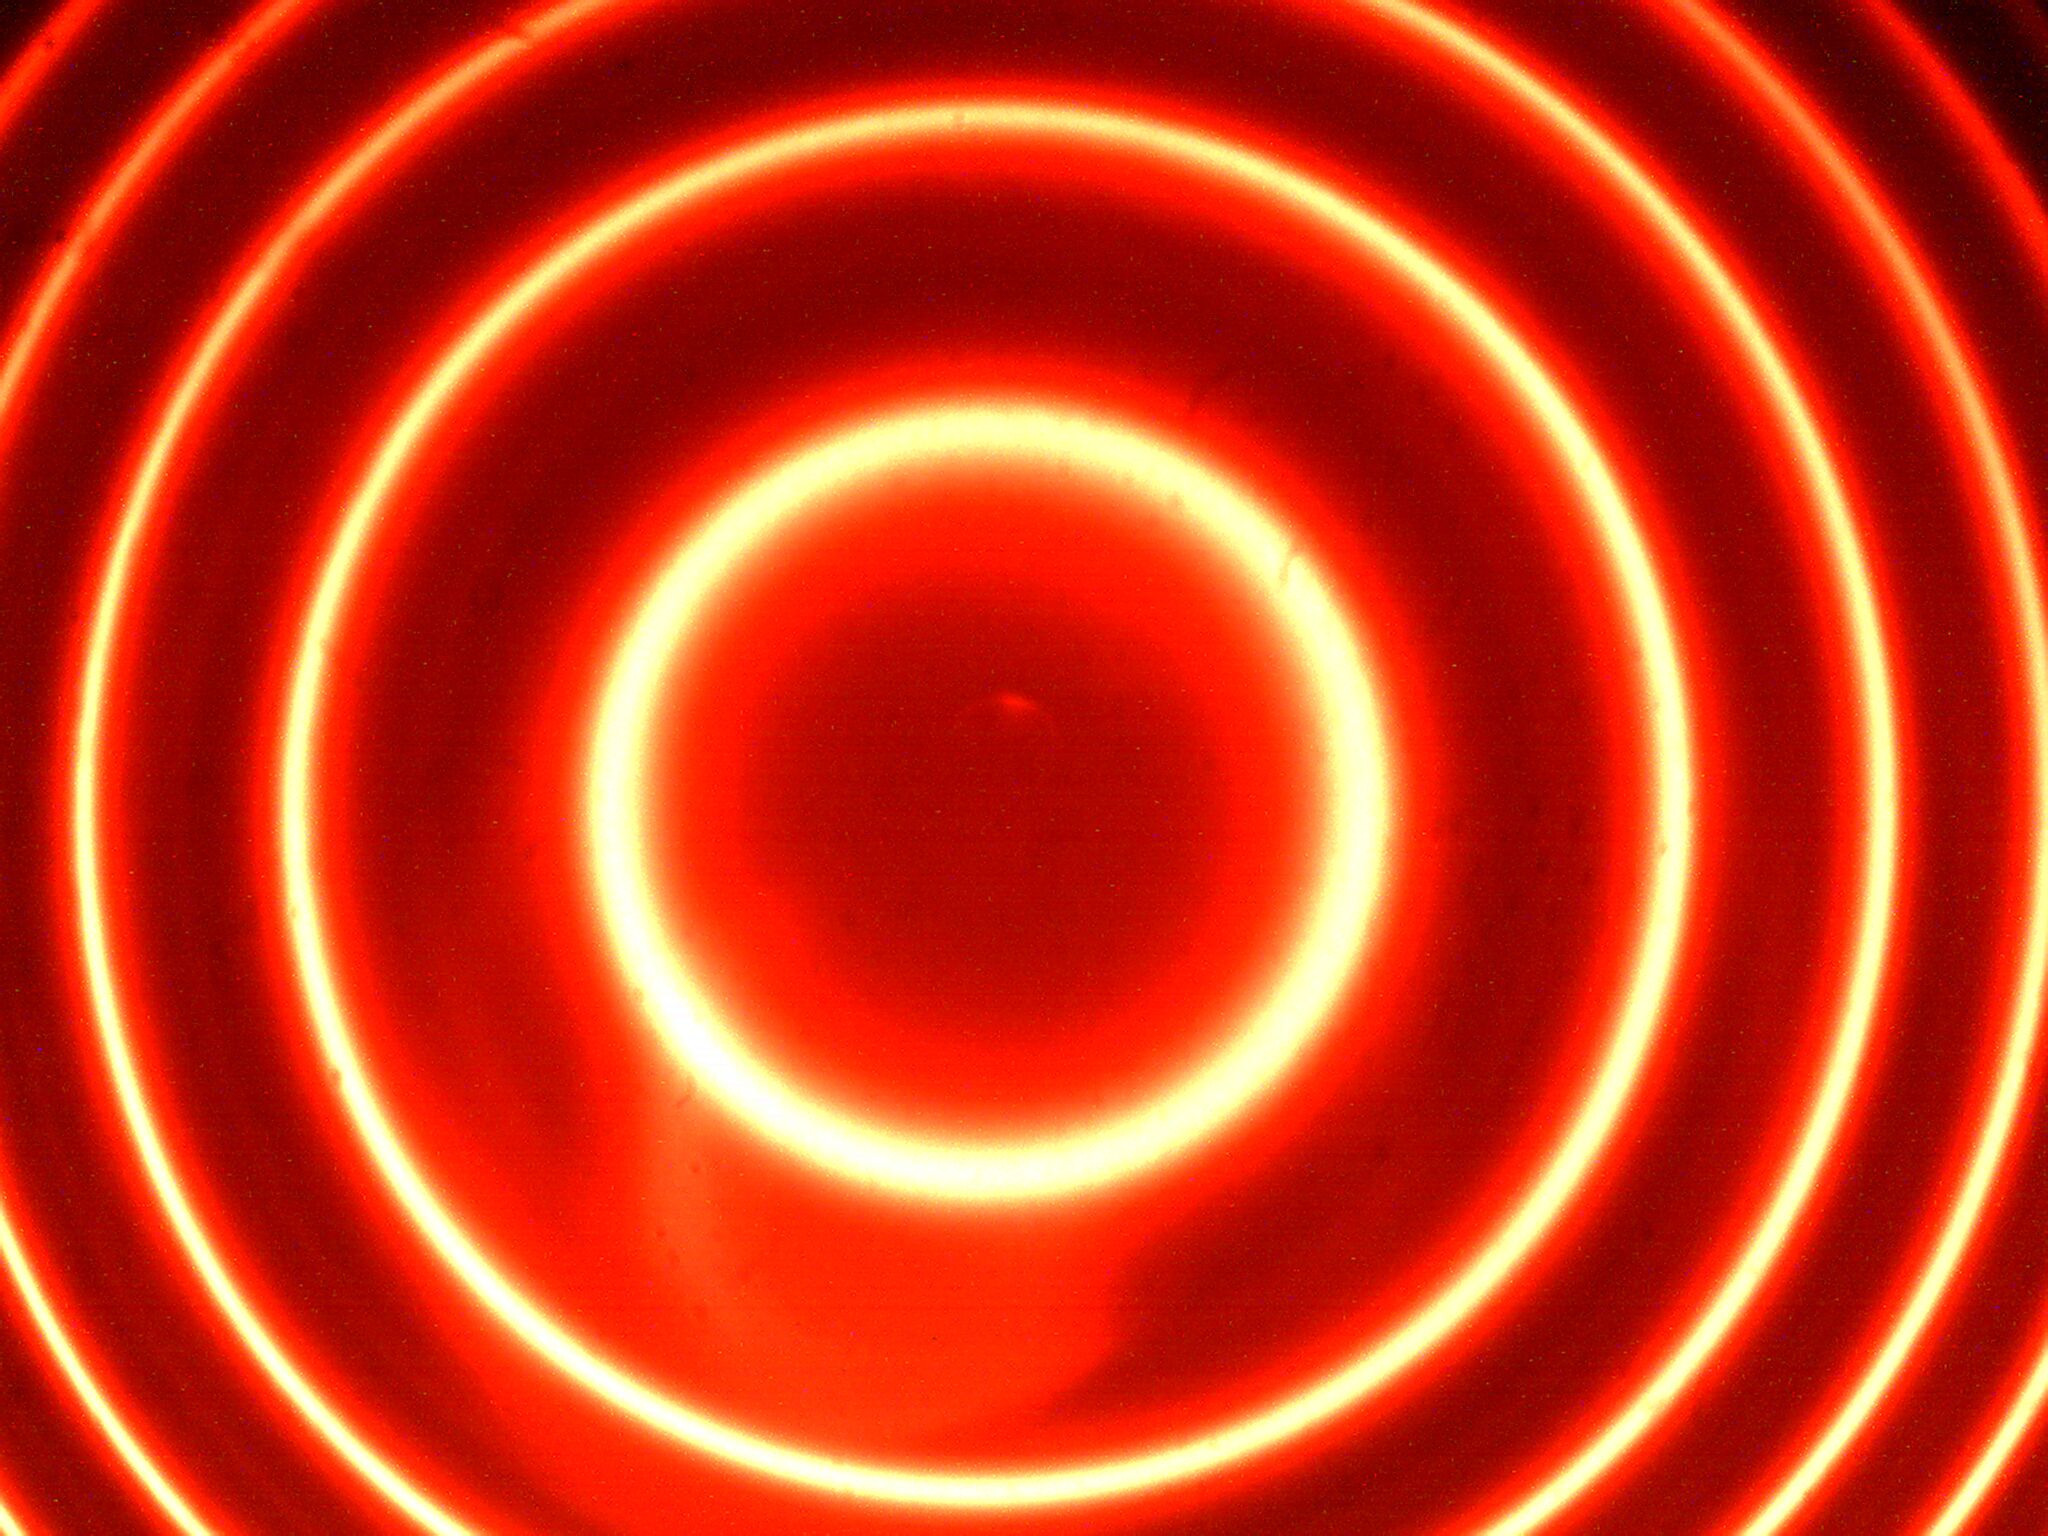
\includegraphics[width=0.55\textwidth]{images/Capture_810.bmp.jpg}
	    \caption{Überbeleuchtete Interferenzringe von rote Emissionslinie}
	    \label{fig:red-fringes}
	    \vspace{-1em}
	\end{figure}

	Nach Anpassung der Beleuchtung im Program.
	\begin{figure}[!ht]
	    \centering
	    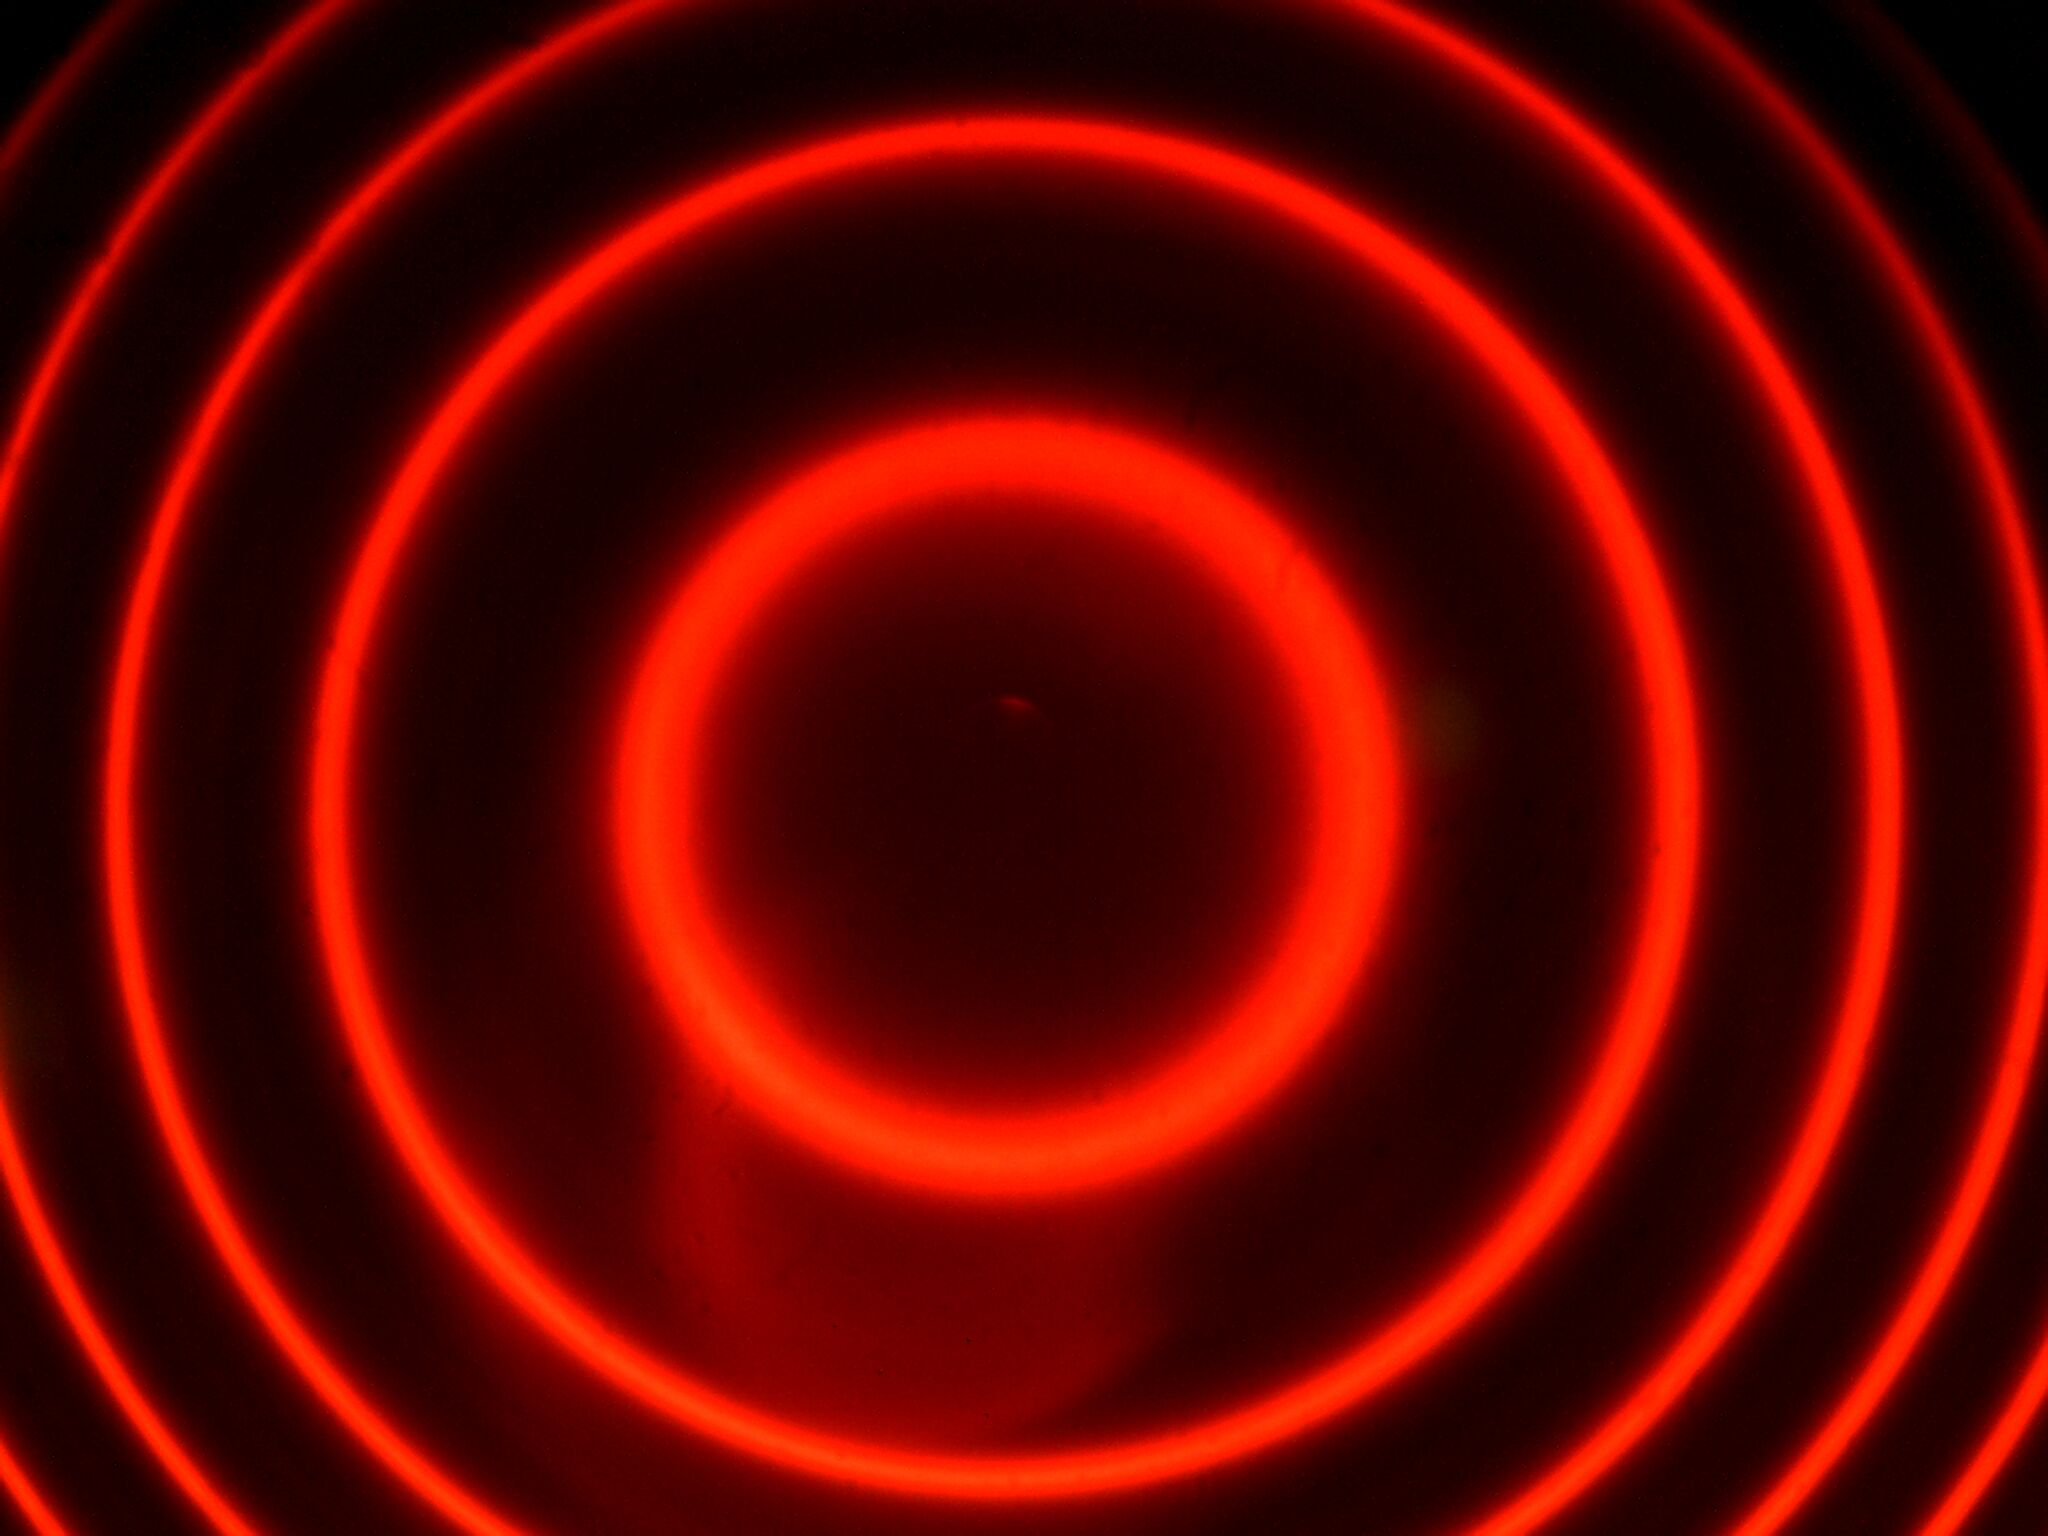
\includegraphics[width=0.45\textwidth]{images/Capture_811.bmp.jpg}
	    \hspace{1em}
	    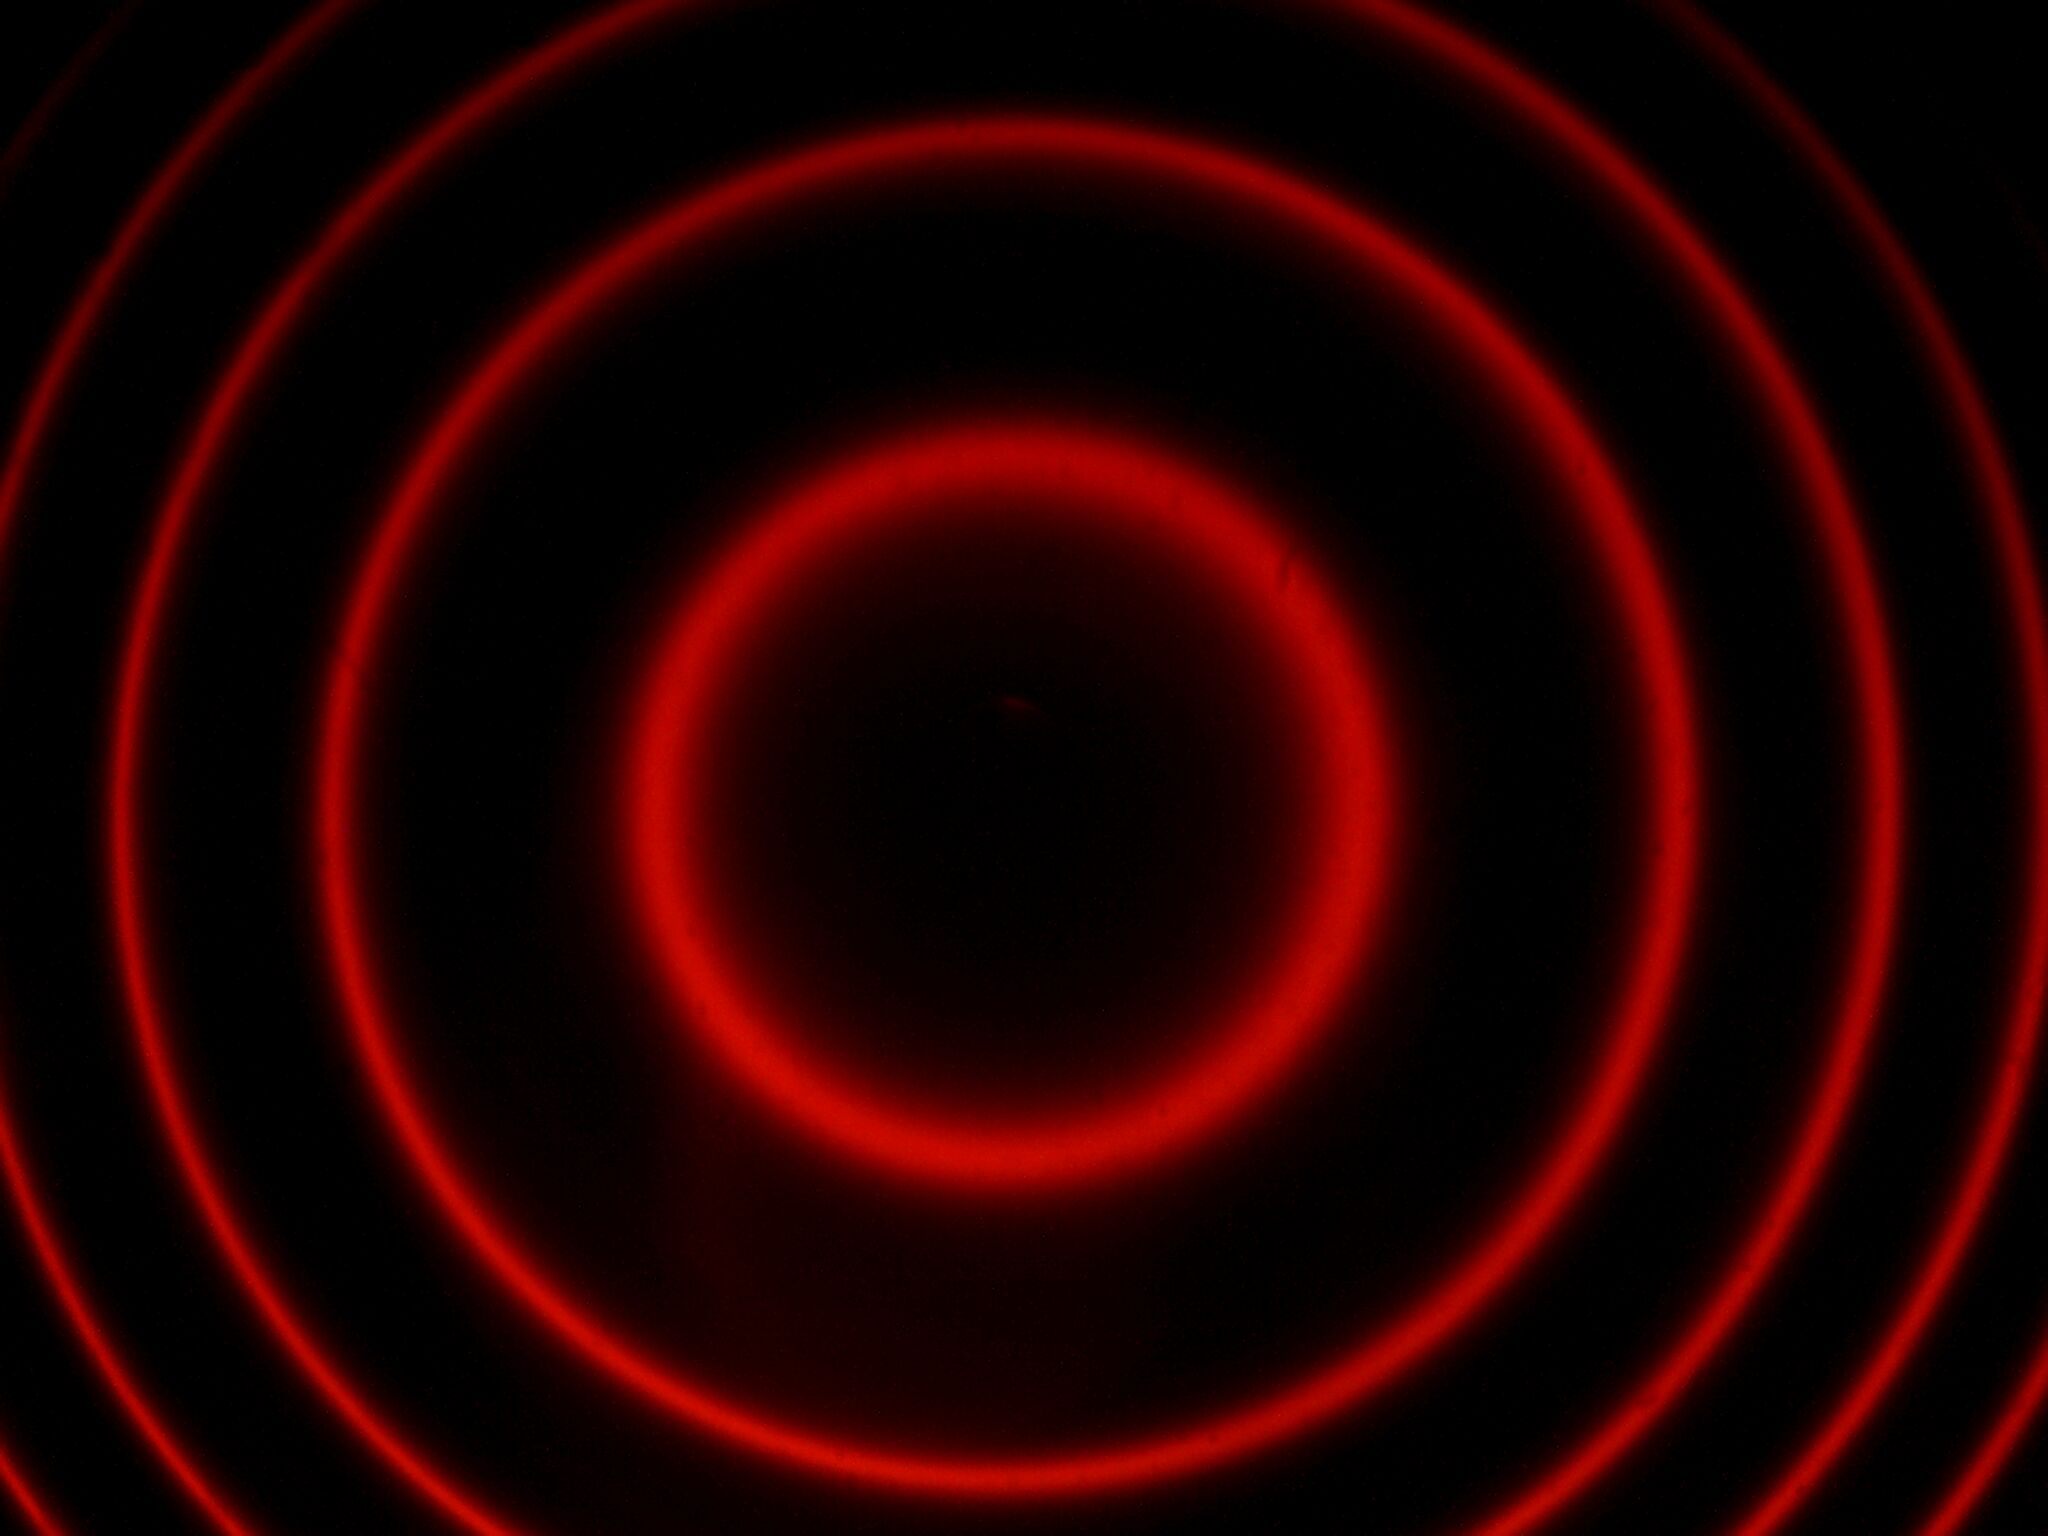
\includegraphics[width=0.45\textwidth]{images/Capture_812.bmp.jpg}
	    \caption{Interferenzringe von rote Emissionslinie. Ohne Polarisationsfilter (Links). Mit Polarisationsfilter (Rechts)}
	    \label{fig:red-fringes-pol}
	    \vspace{-0.5em}
	\end{figure}
	\begin{figure}[!ht]
	    \centering
	    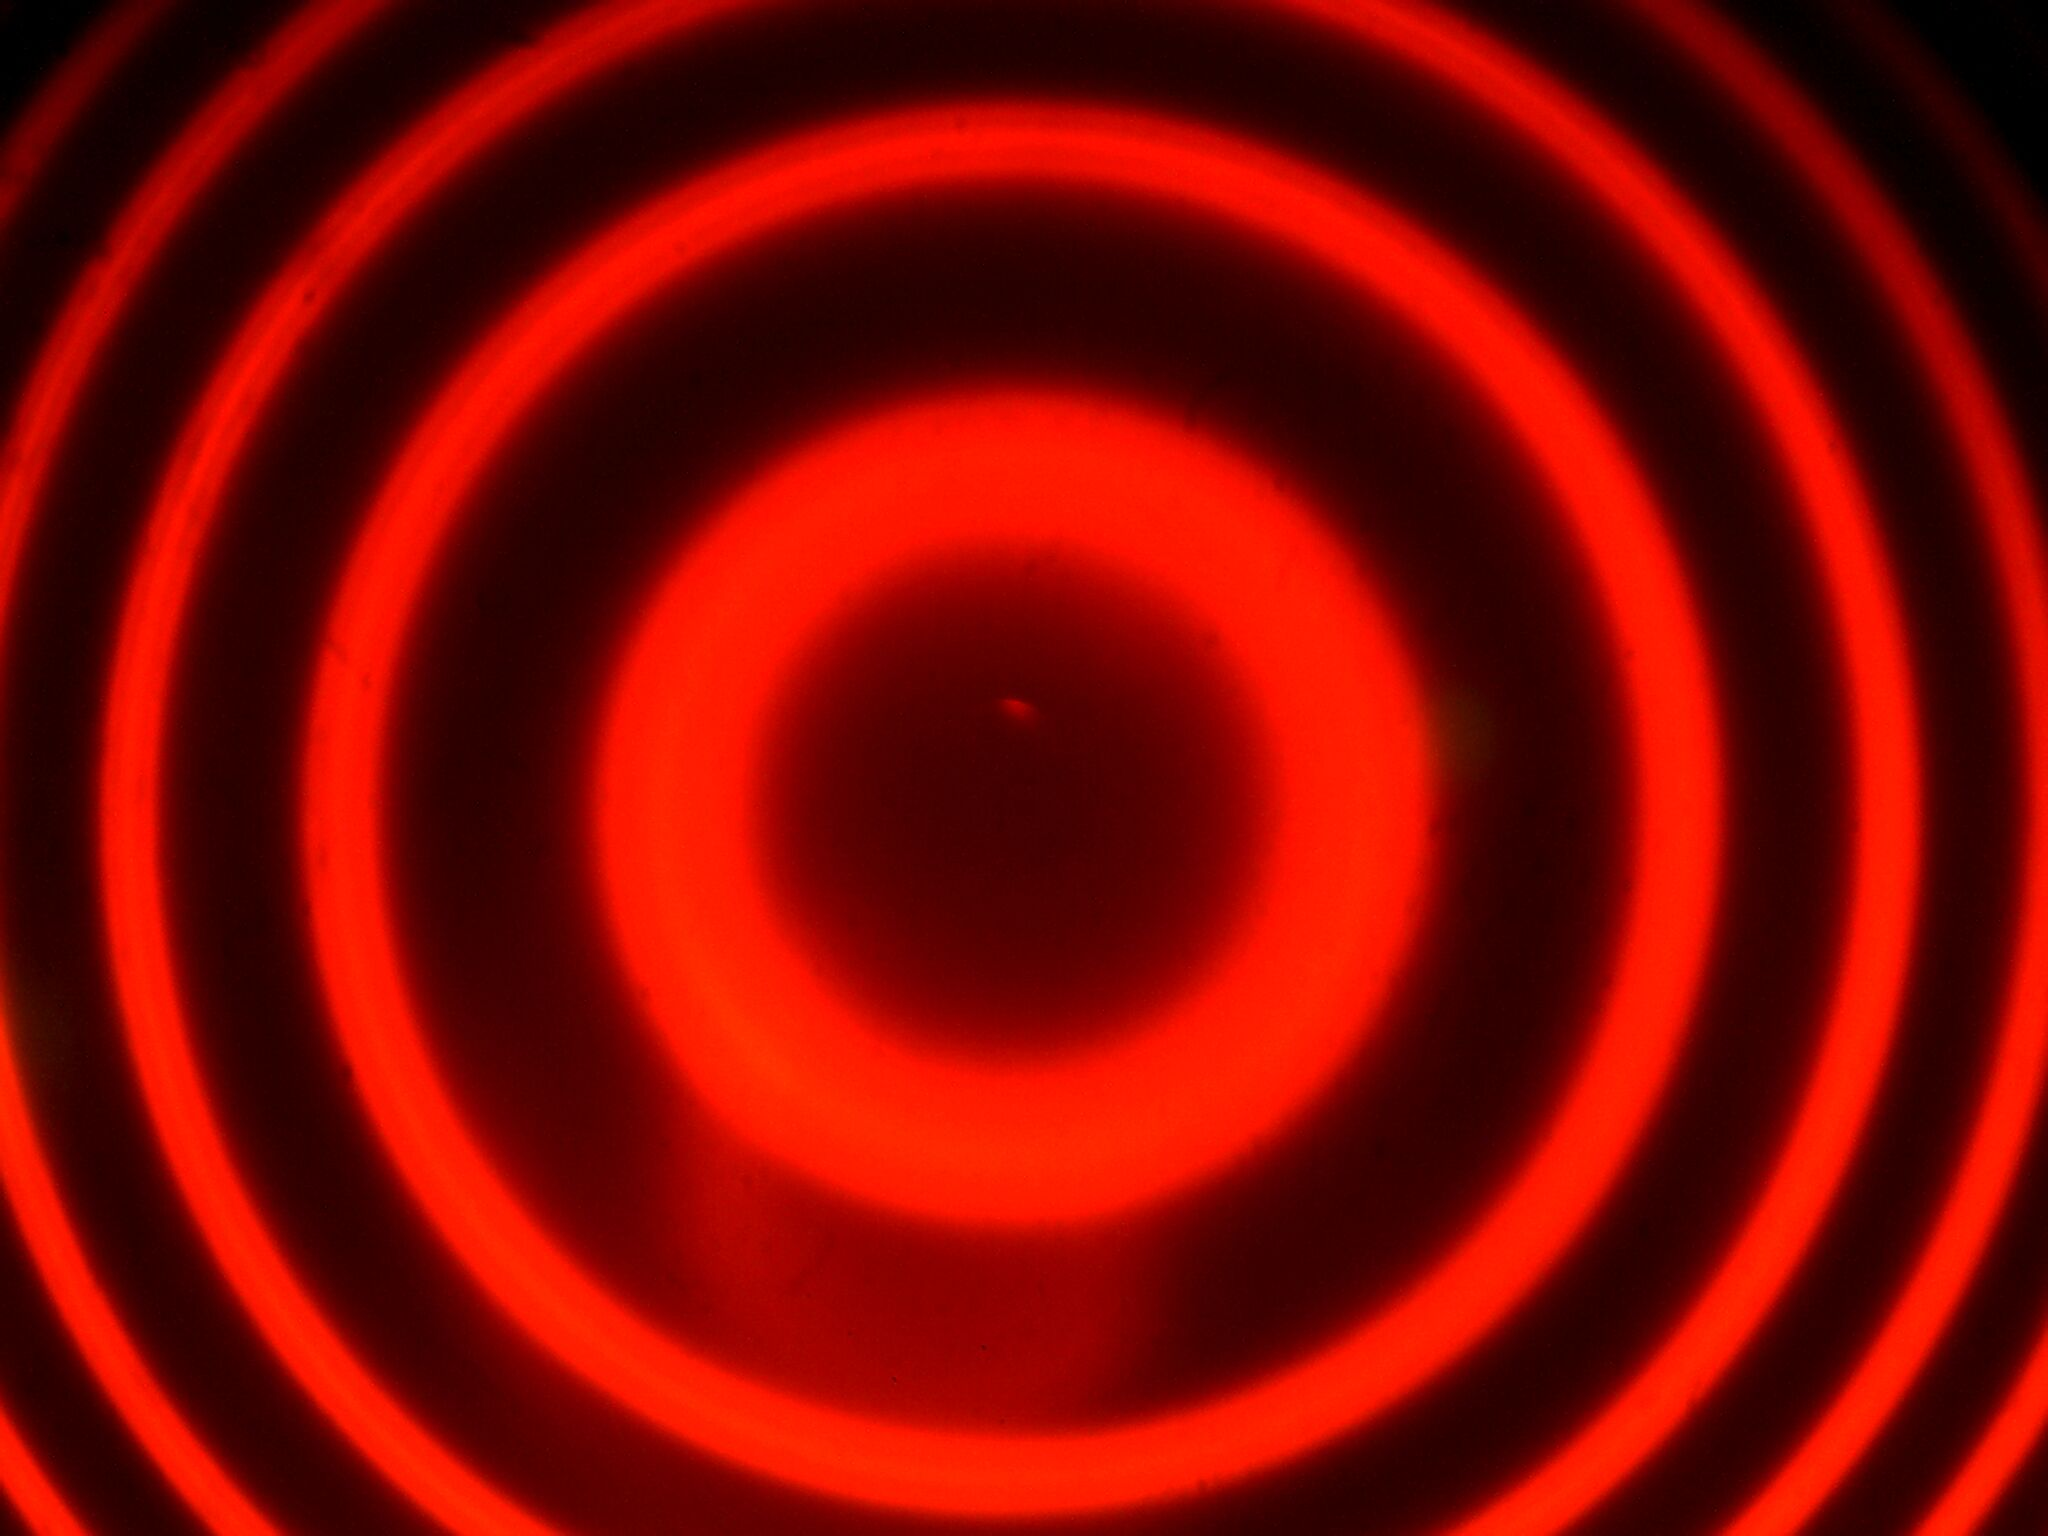
\includegraphics[width=0.45\textwidth]{images/Capture_814.bmp.jpg}
	    \hspace{1em}
	    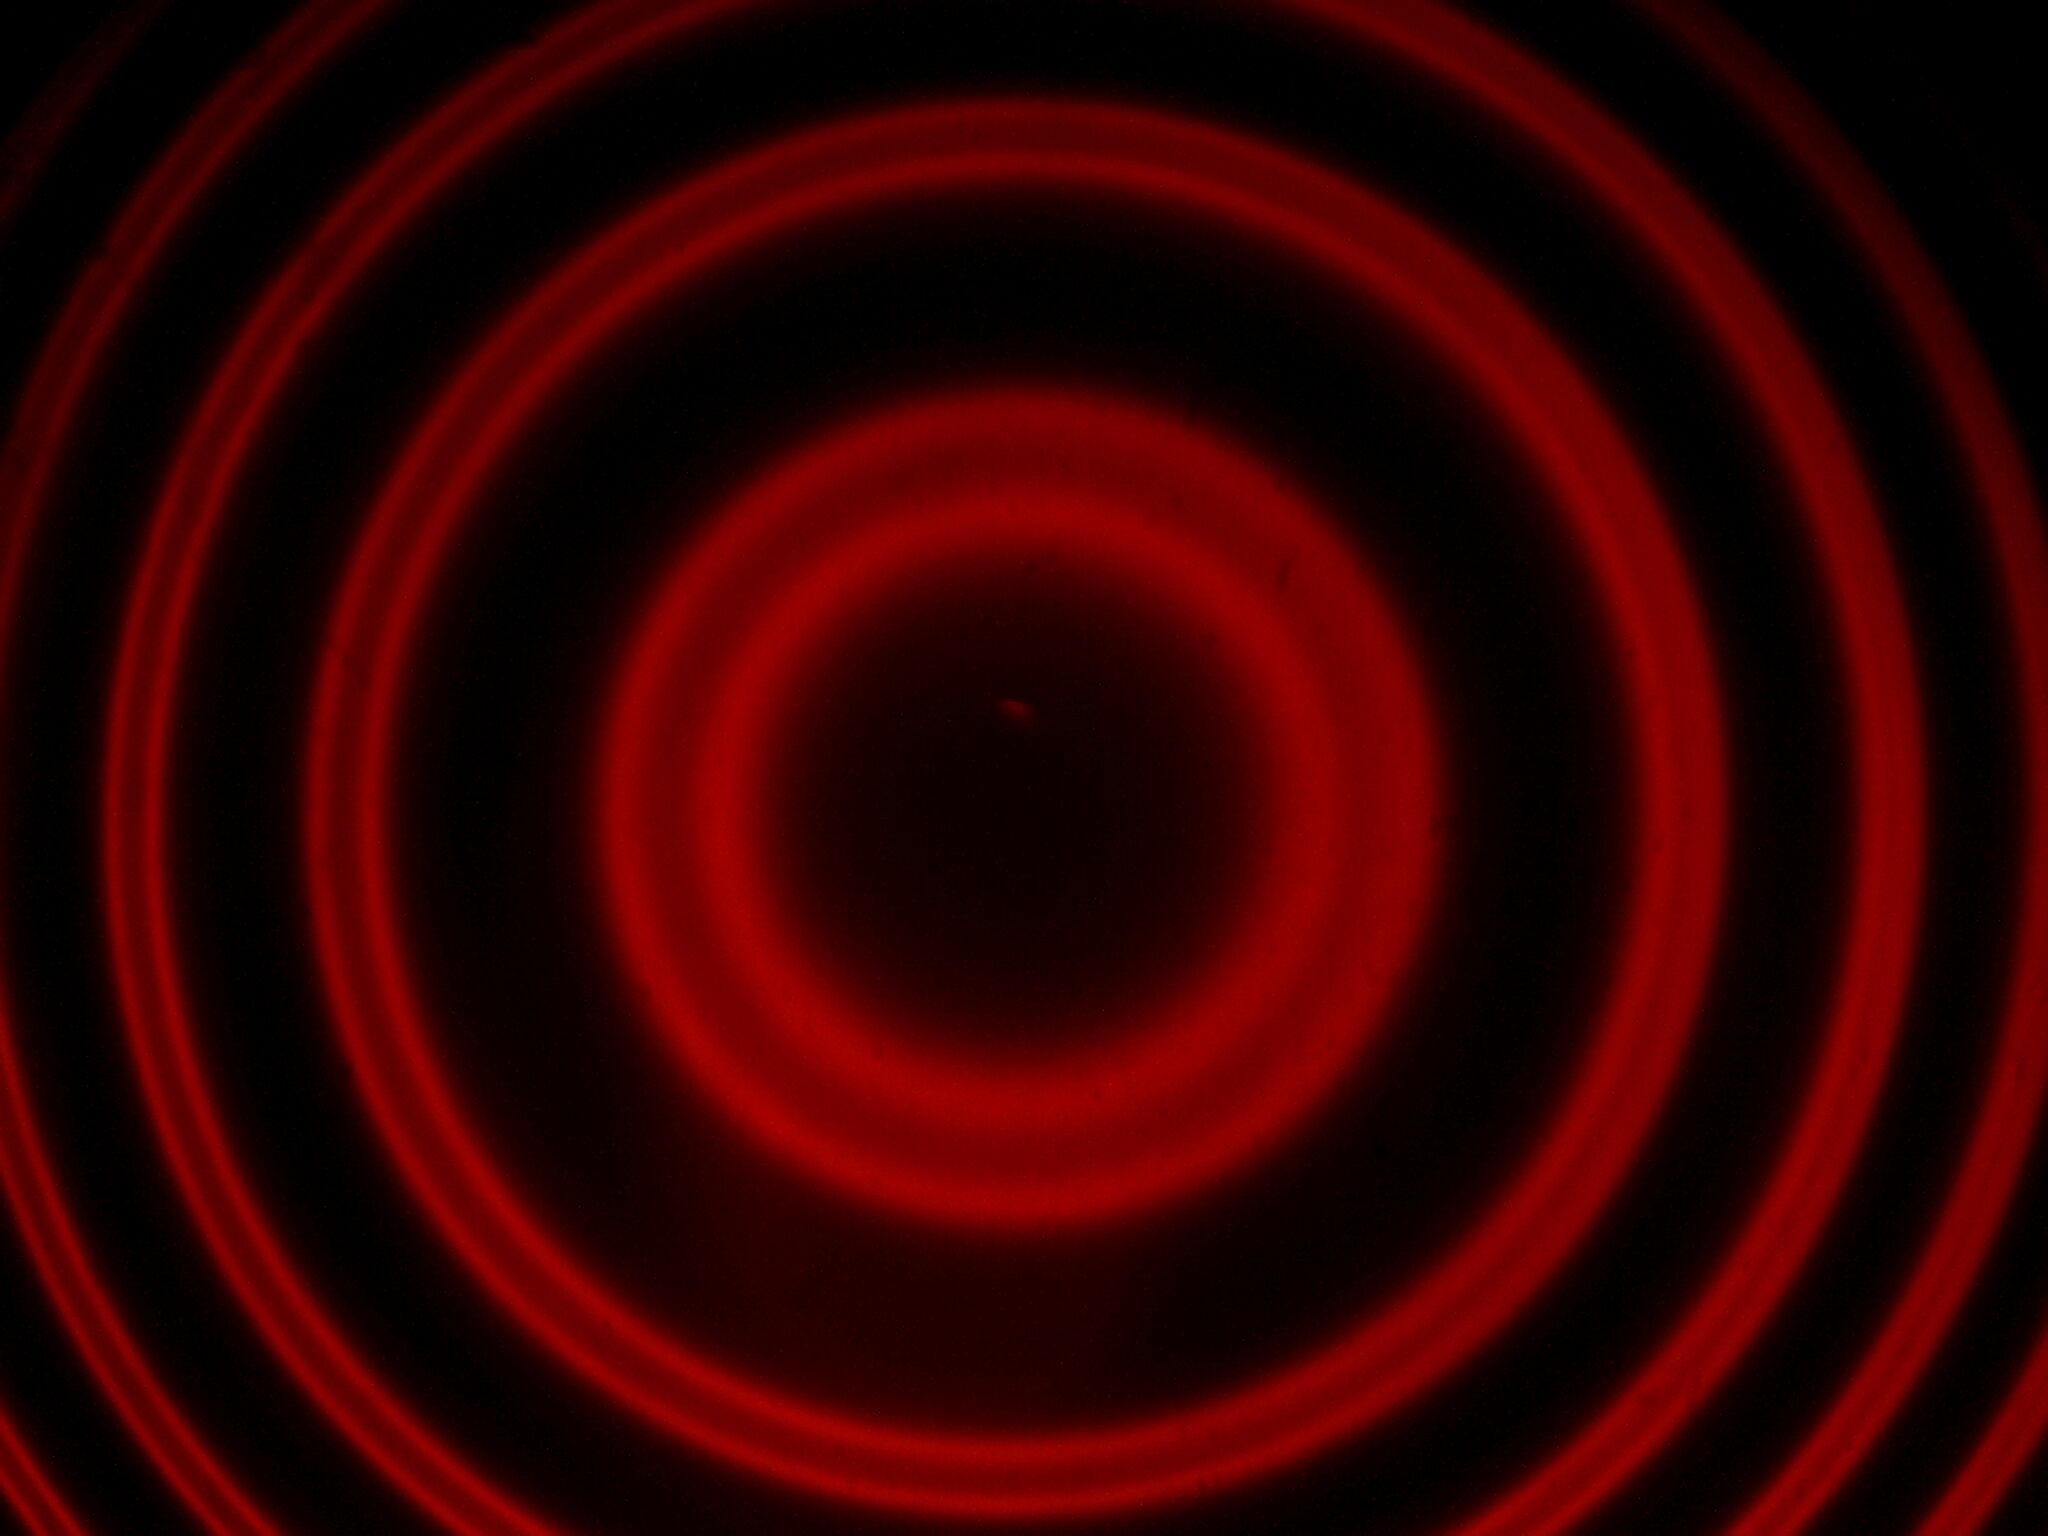
\includegraphics[width=0.45\textwidth]{images/Capture_813.bmp.jpg}
	    \caption{Interferenzringe von rote Emissionslinie im Magnetfeld $B \approx 2\text{ - }3 \si{\ampere}$. Ohne Polarisationsfilter (Links). Mit Polarisationsfilter (Rechts)}
	    \label{fig:red-fringes-pol-B}
	    \vspace{-0.5em}
	\end{figure}
	\begin{figure}[!ht]
	    \centering
	    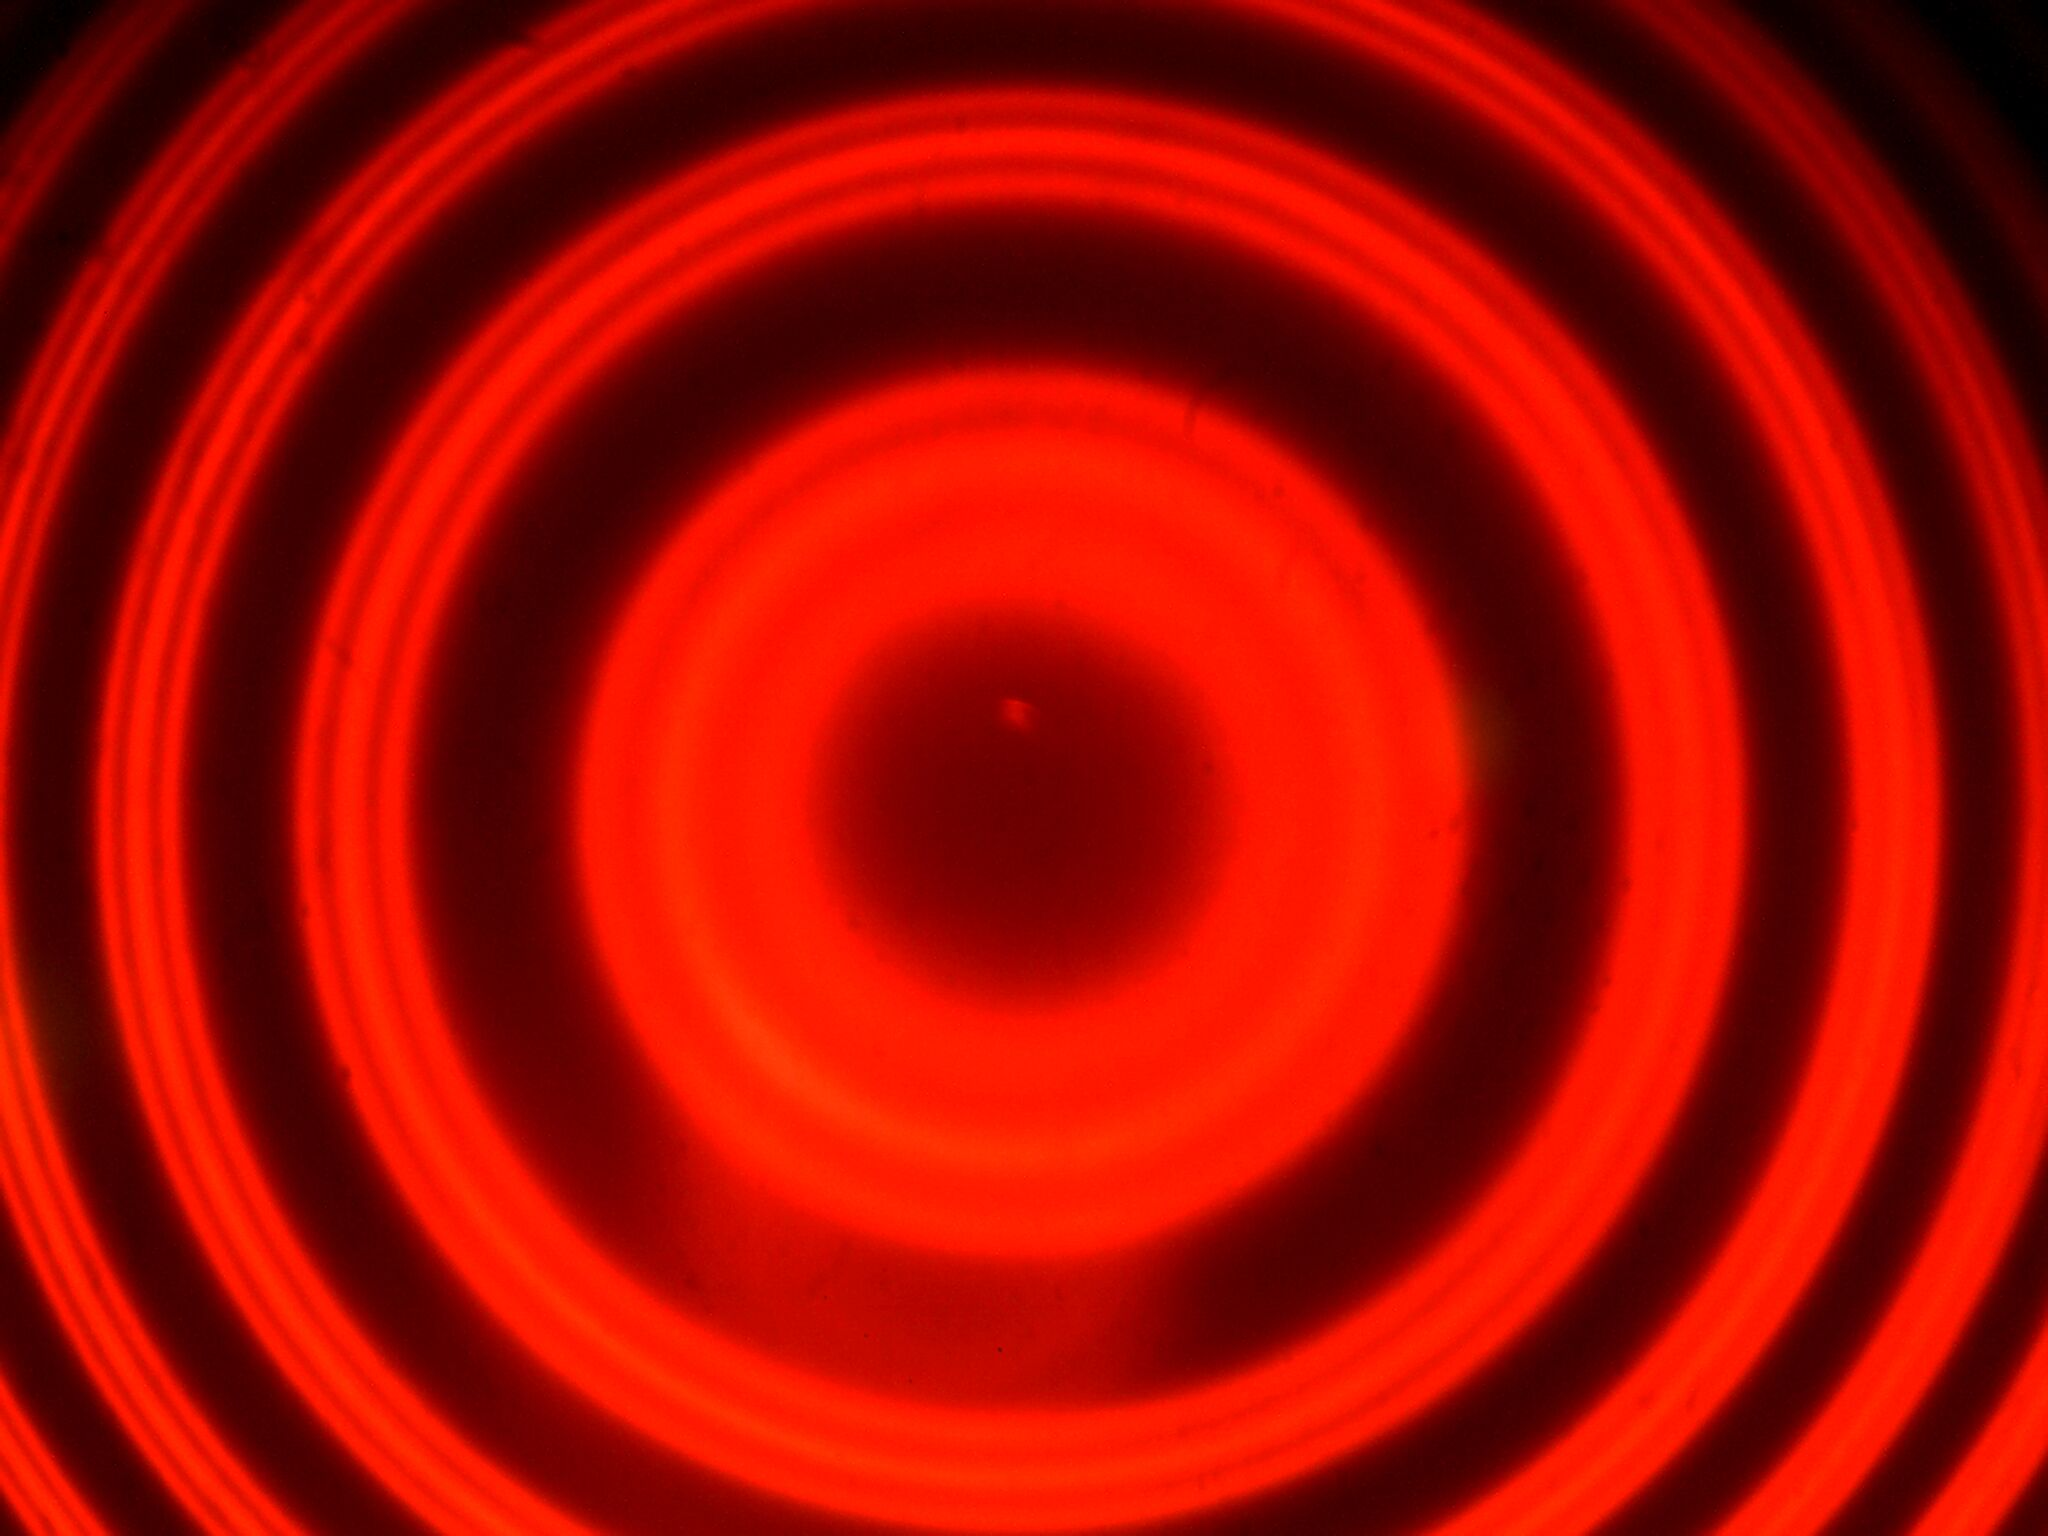
\includegraphics[width=0.45\textwidth]{images/Capture_816.bmp.jpg}
	    \hspace{1em}
	    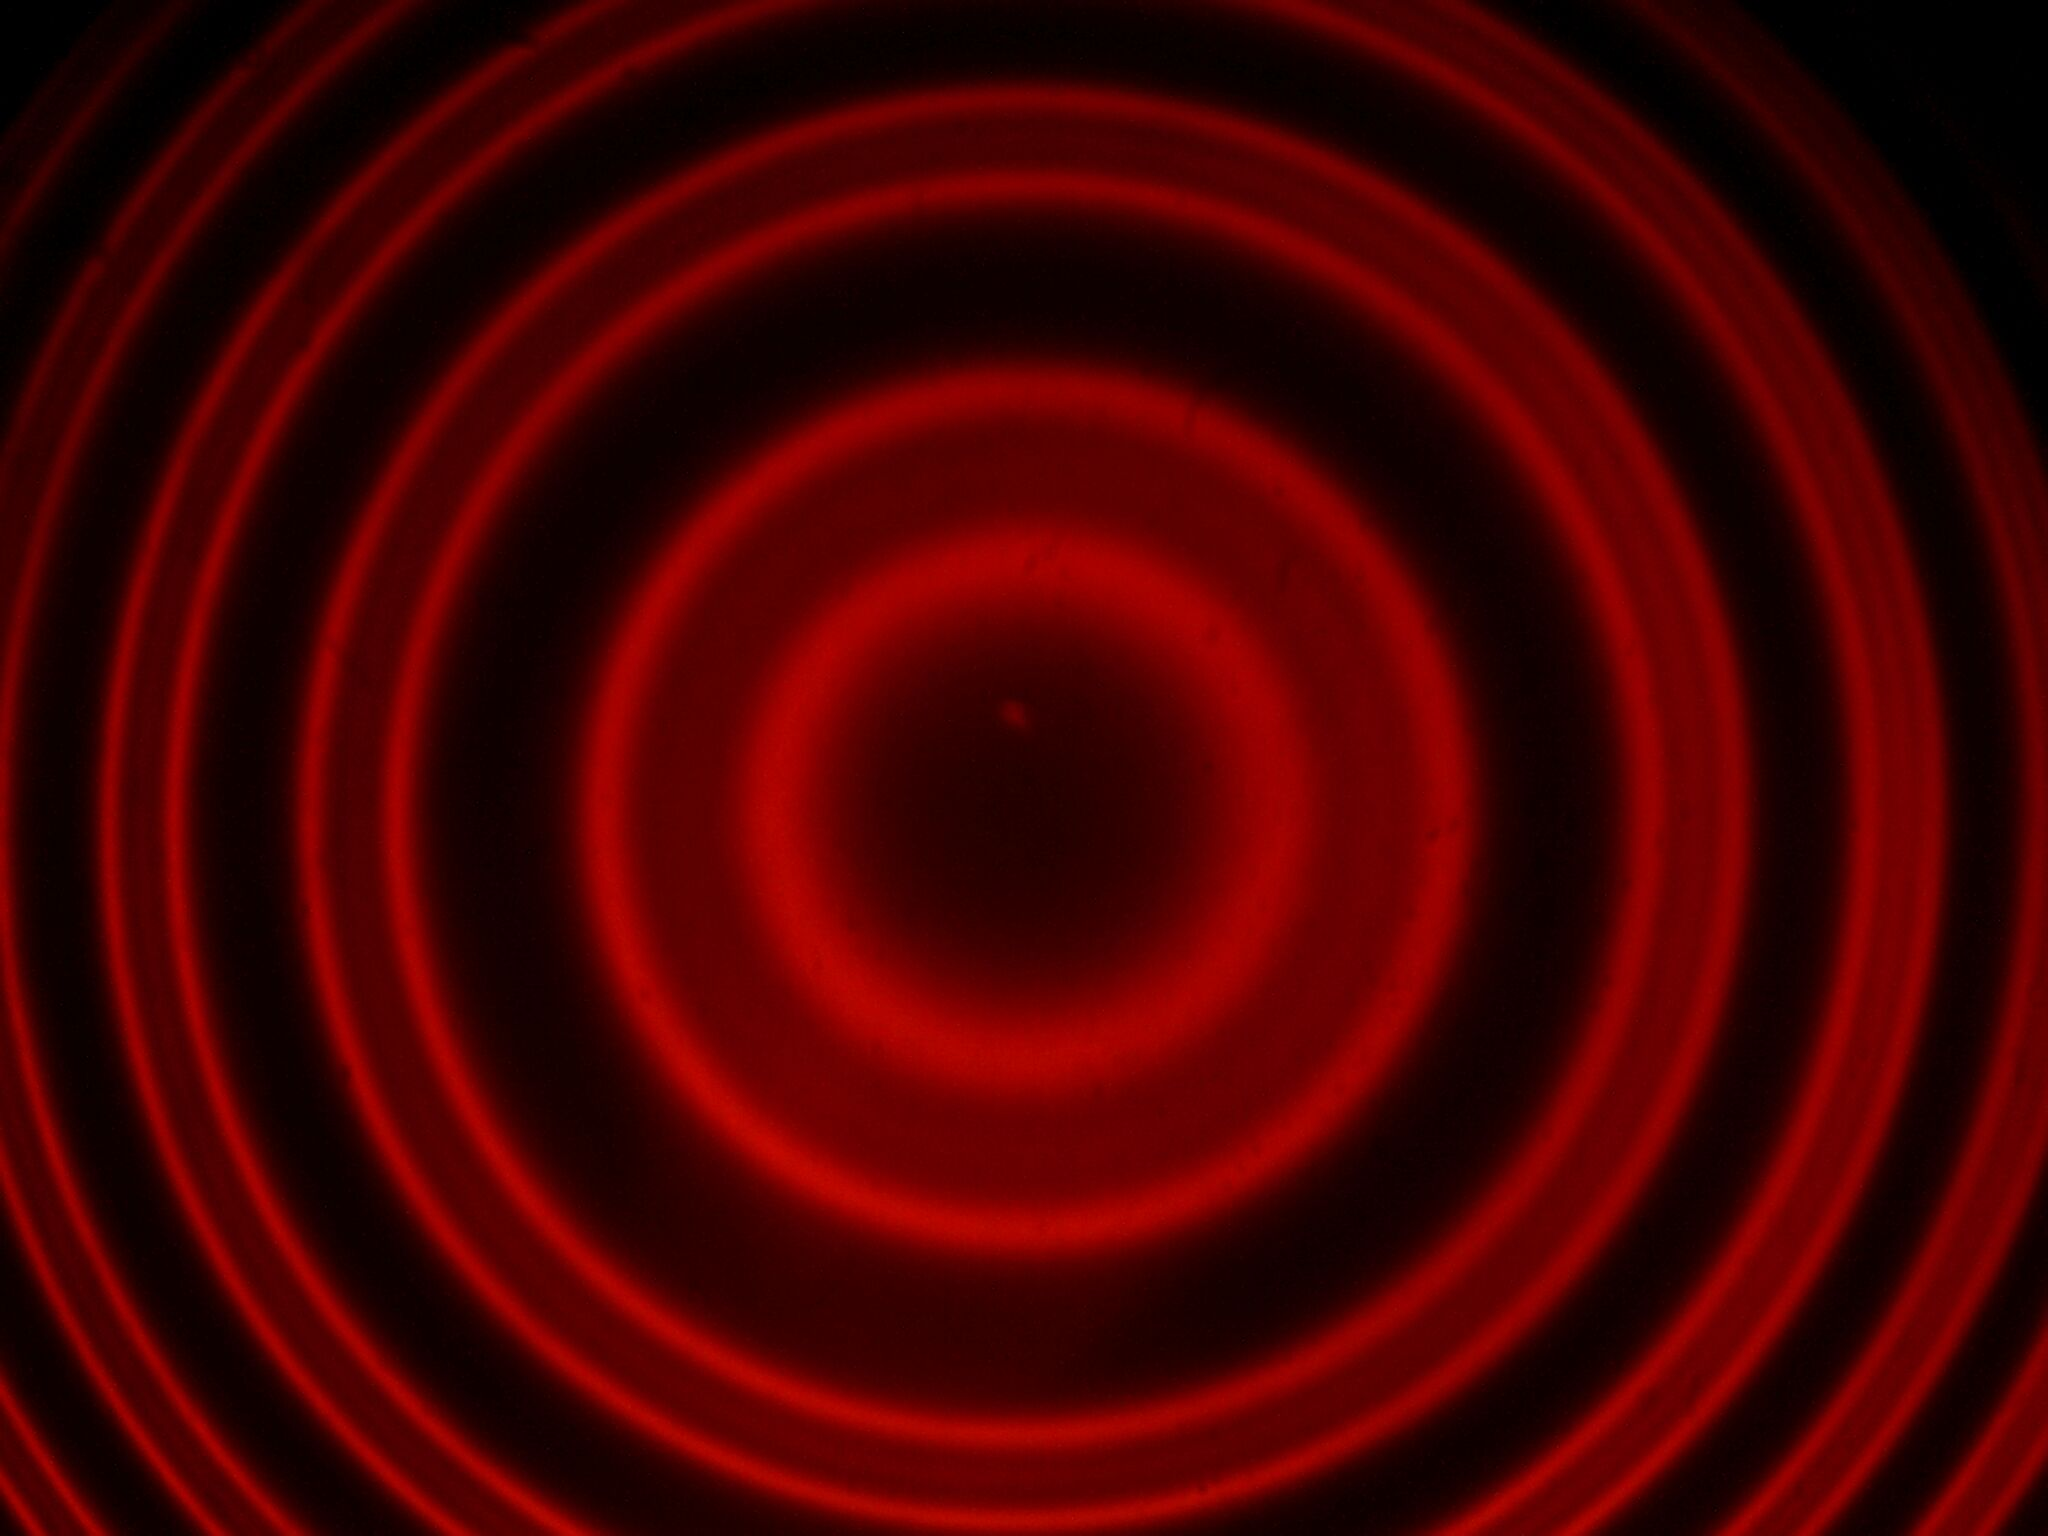
\includegraphics[width=0.45\textwidth]{images/Capture_815.bmp.jpg}
	    \caption{Interferenzringe von rote Emissionslinie im Magnetfeld $B \approx  \SI{6}{\ampere}$. Ohne Polarisationsfilter (Links). Mit Polarisationsfilter (Rechts)}
	    \label{fig:red-fringes-pol-B-big}
	    \vspace{-0.5em}
	\end{figure}
	\newpage
	\begin{figure}[!ht]
	    \centering
	   	\begin{subfigure}{0.48\textwidth}
			\centering
			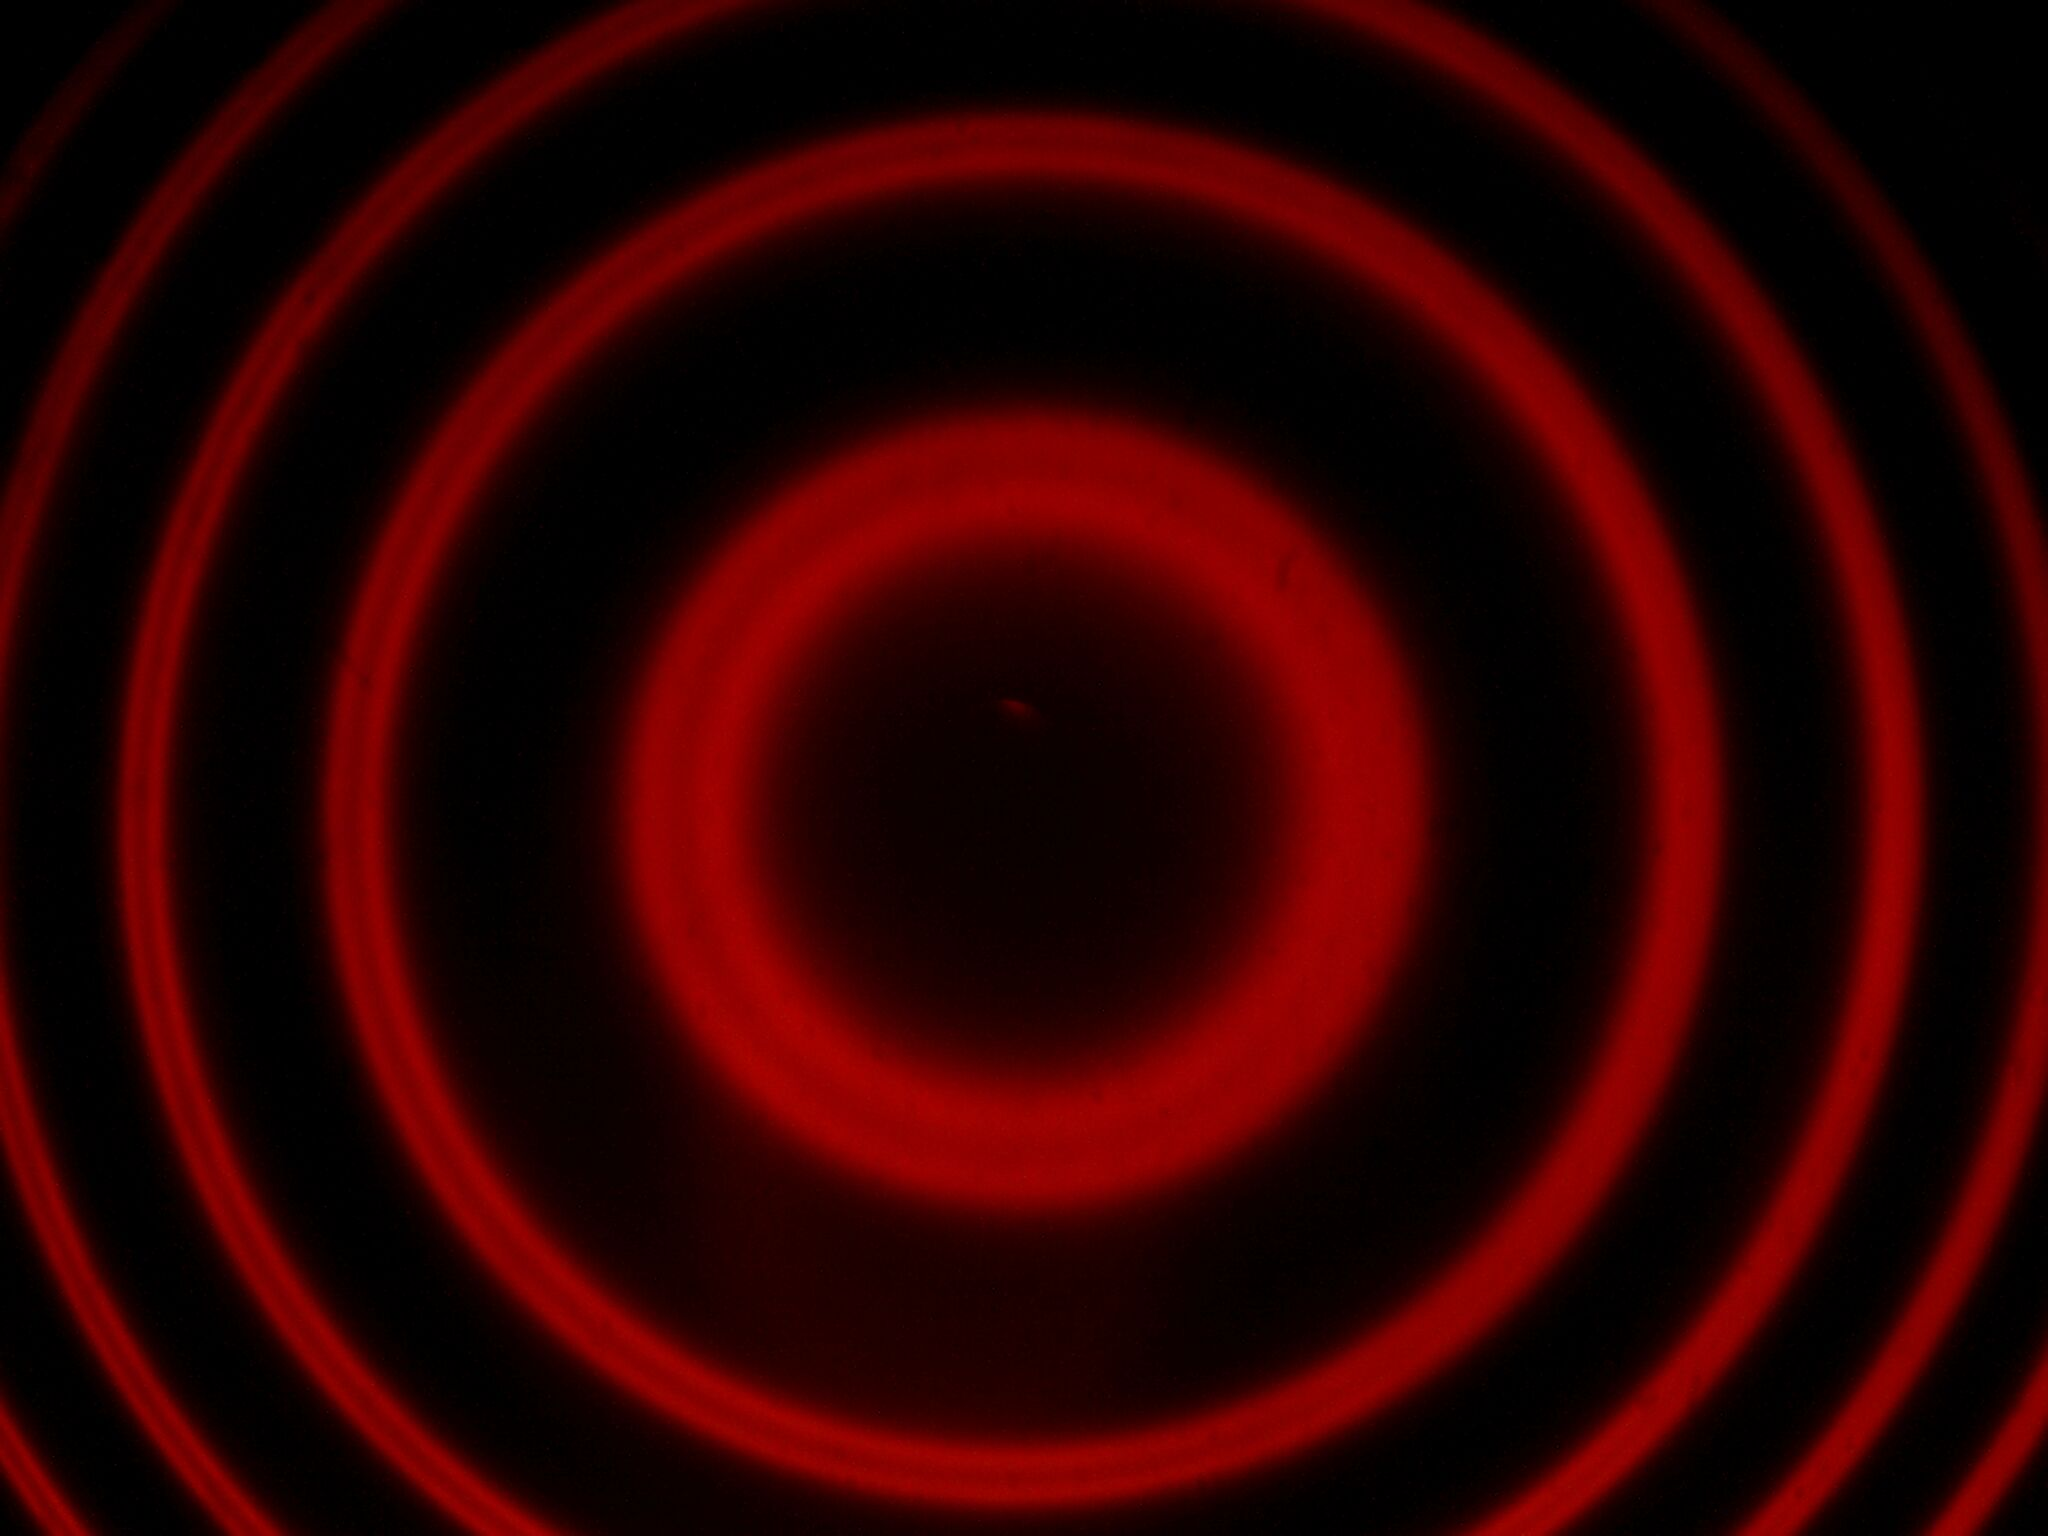
\includegraphics[width=\textwidth]{images/Capture_817.bmp.jpg}
			\caption{$I = \SI{2.495(5)}{\ampere}$}
			\label{fig:red_I2.495}
			\vspace{0.5\baselineskip}
		\end{subfigure}
		\hfill
		\begin{subfigure}{0.48\textwidth}
			\centering
			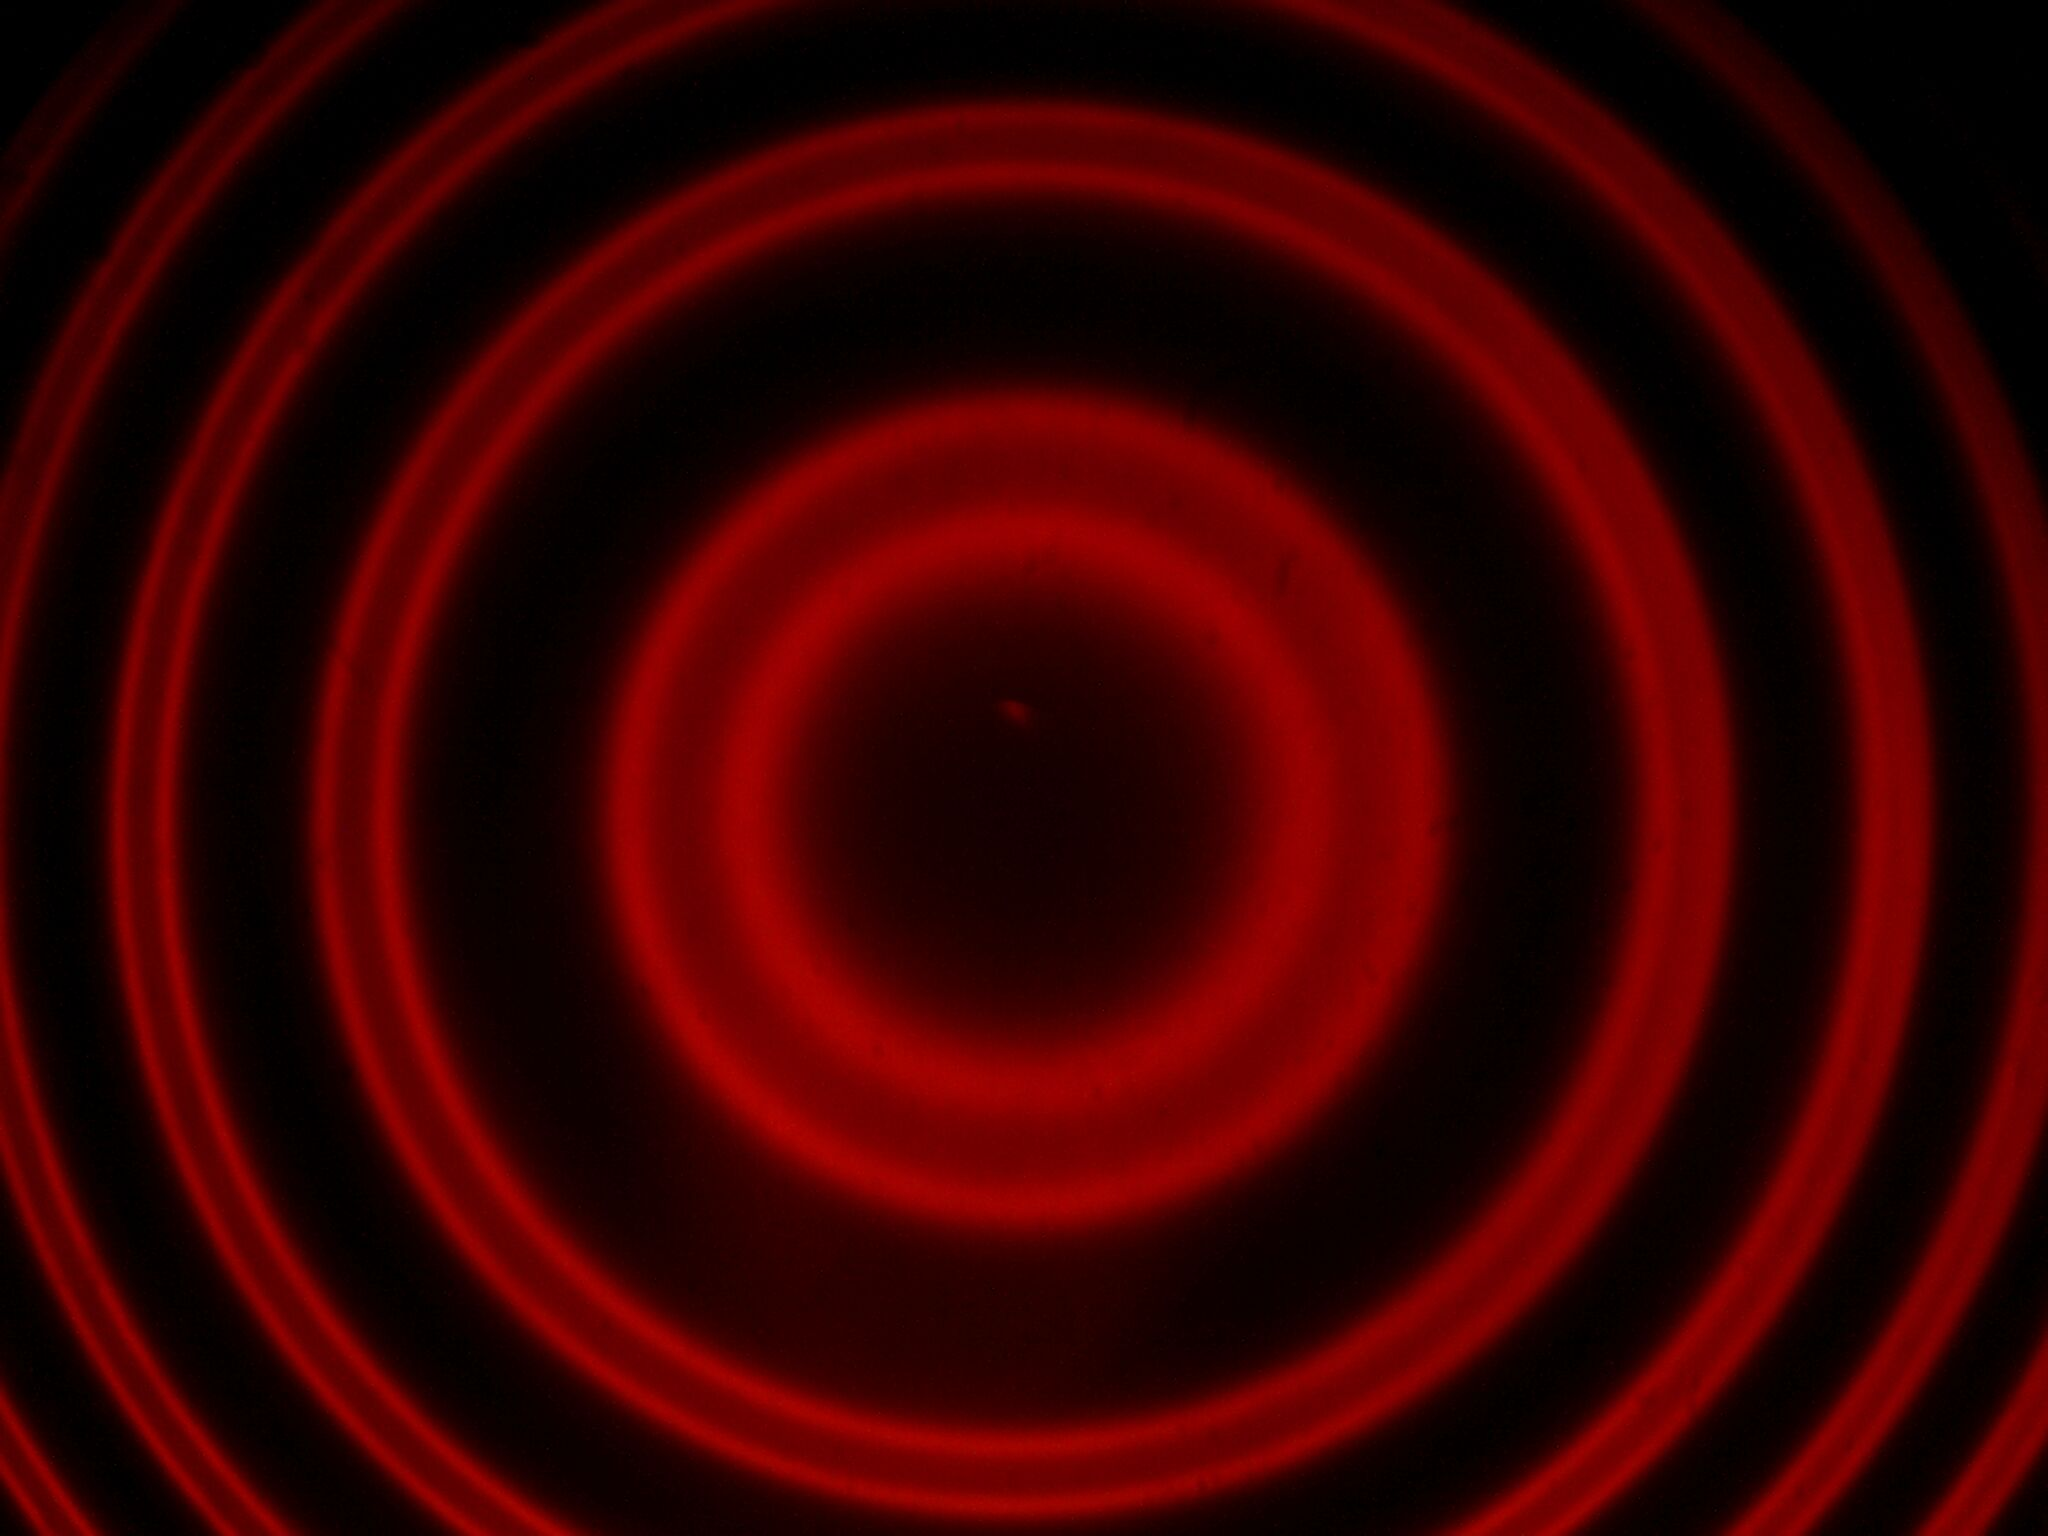
\includegraphics[width=\textwidth]{images/Capture_818.bmp.jpg}
			\caption{$I = \SI{4.190(10)}{\ampere}$}
			\label{fig:red_I4190}
			\vspace{0.5\baselineskip}
		\end{subfigure}
		\begin{subfigure}{0.48\textwidth}
			\centering
			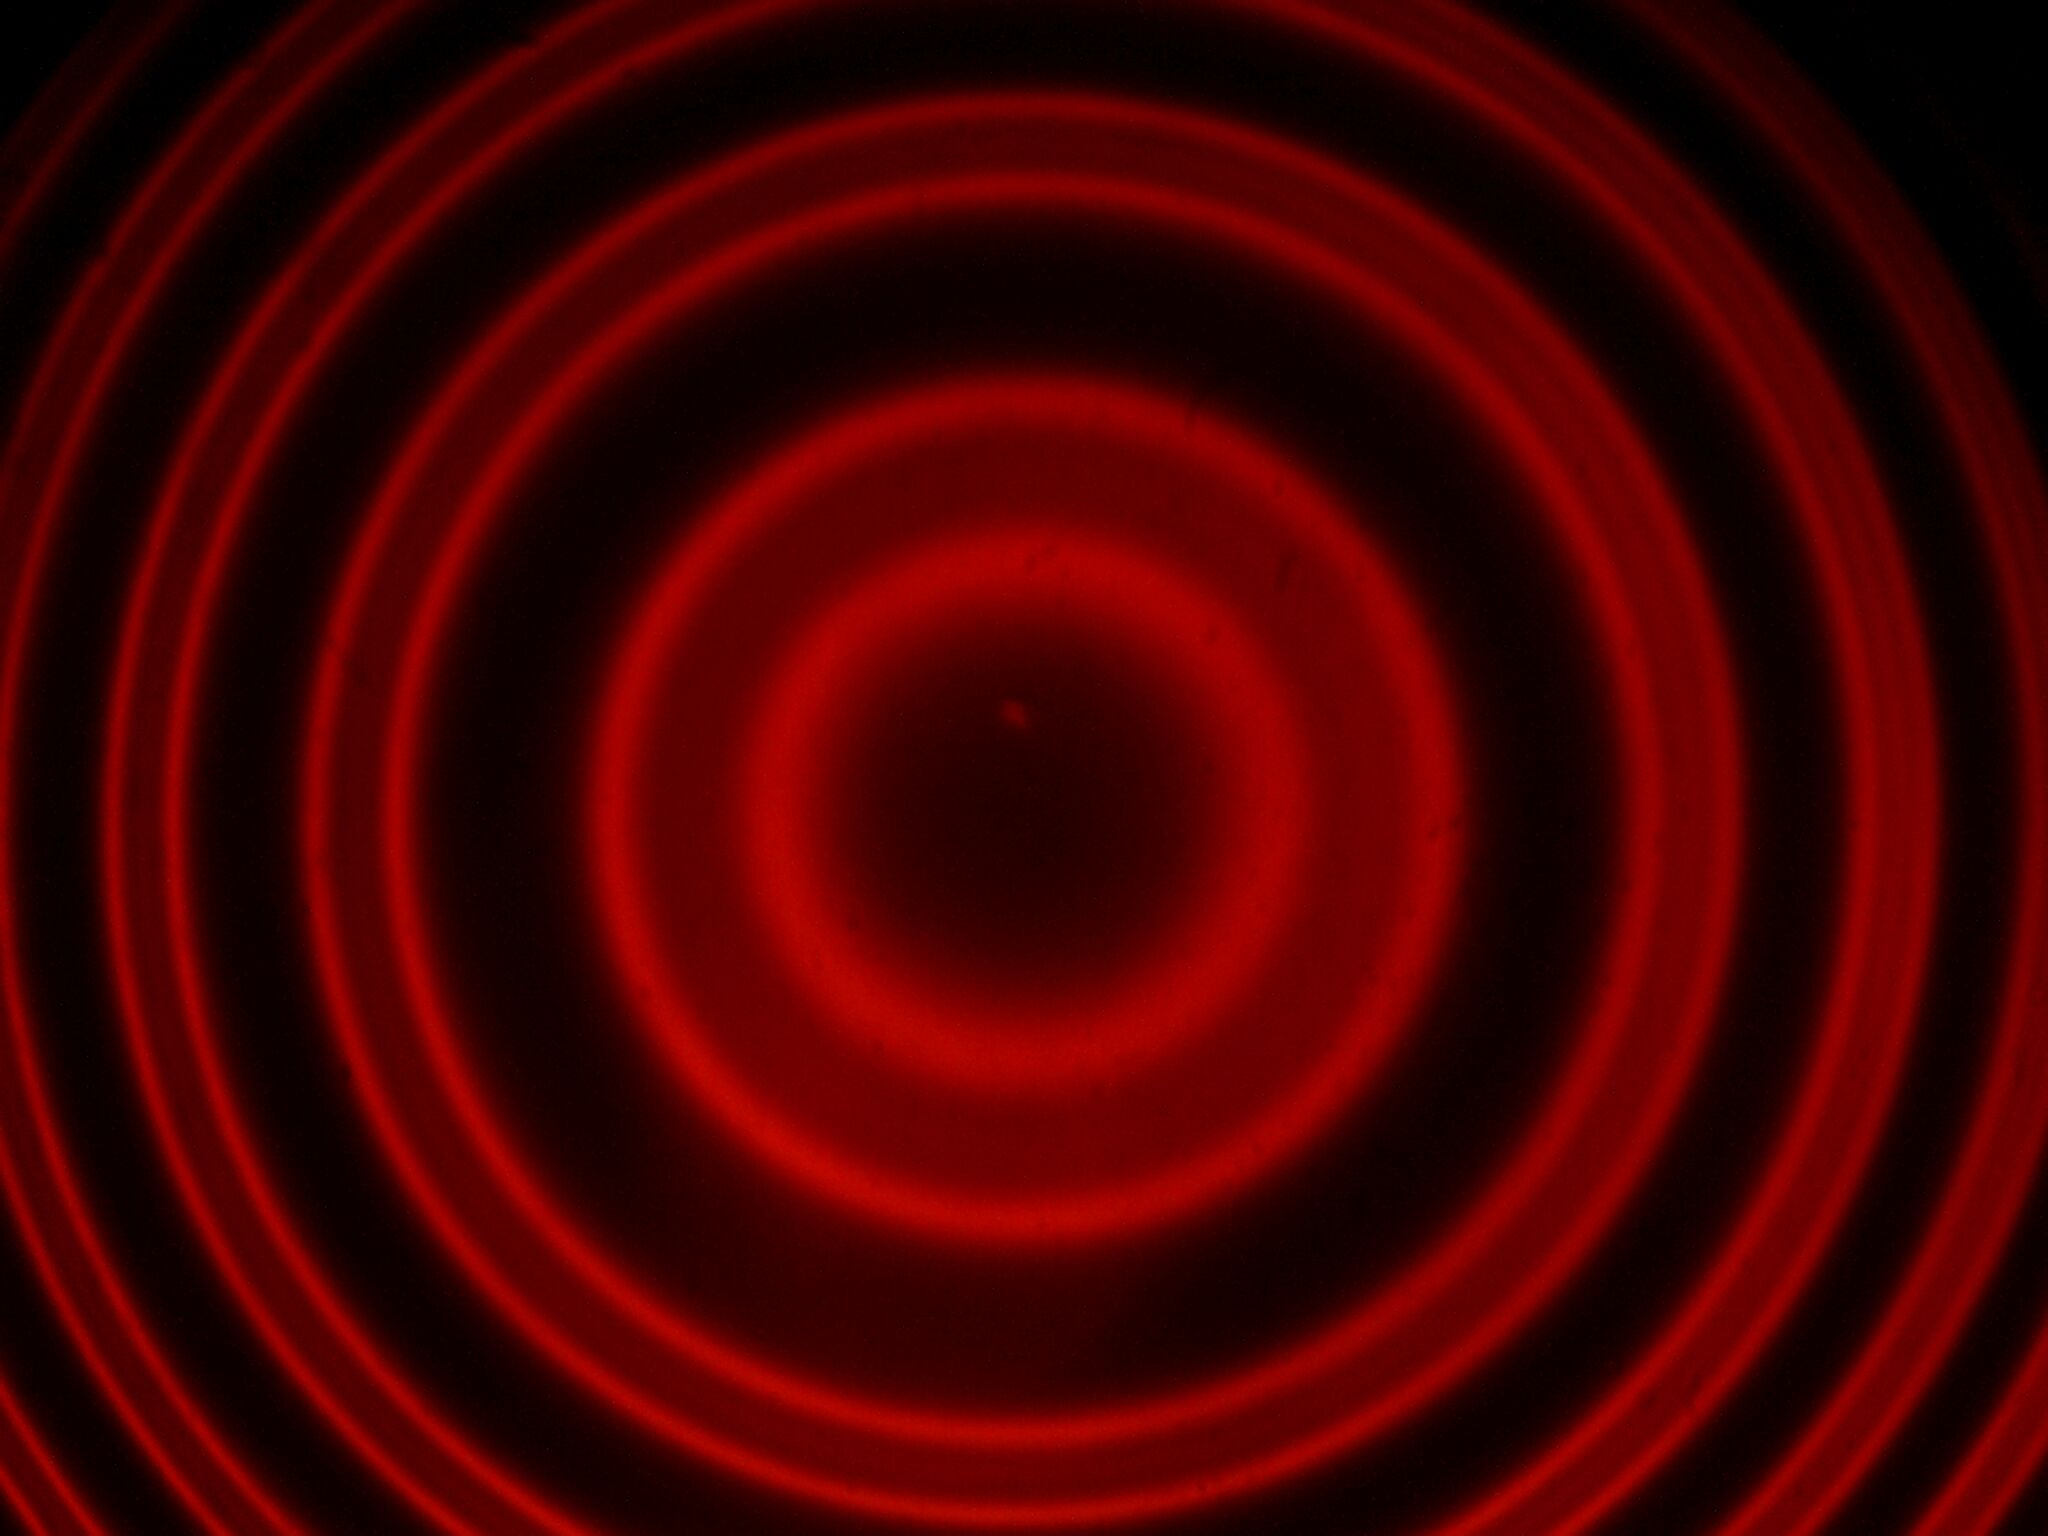
\includegraphics[width=\textwidth]{images/Capture_819.bmp.jpg}
			\caption{$I = \SI{5.662(10)}{\ampere}$}
			\label{fig:red_I5.662}
			\vspace{0.5\baselineskip}
		\end{subfigure}
		\hfill
		\begin{subfigure}{0.48\textwidth}
			\centering
			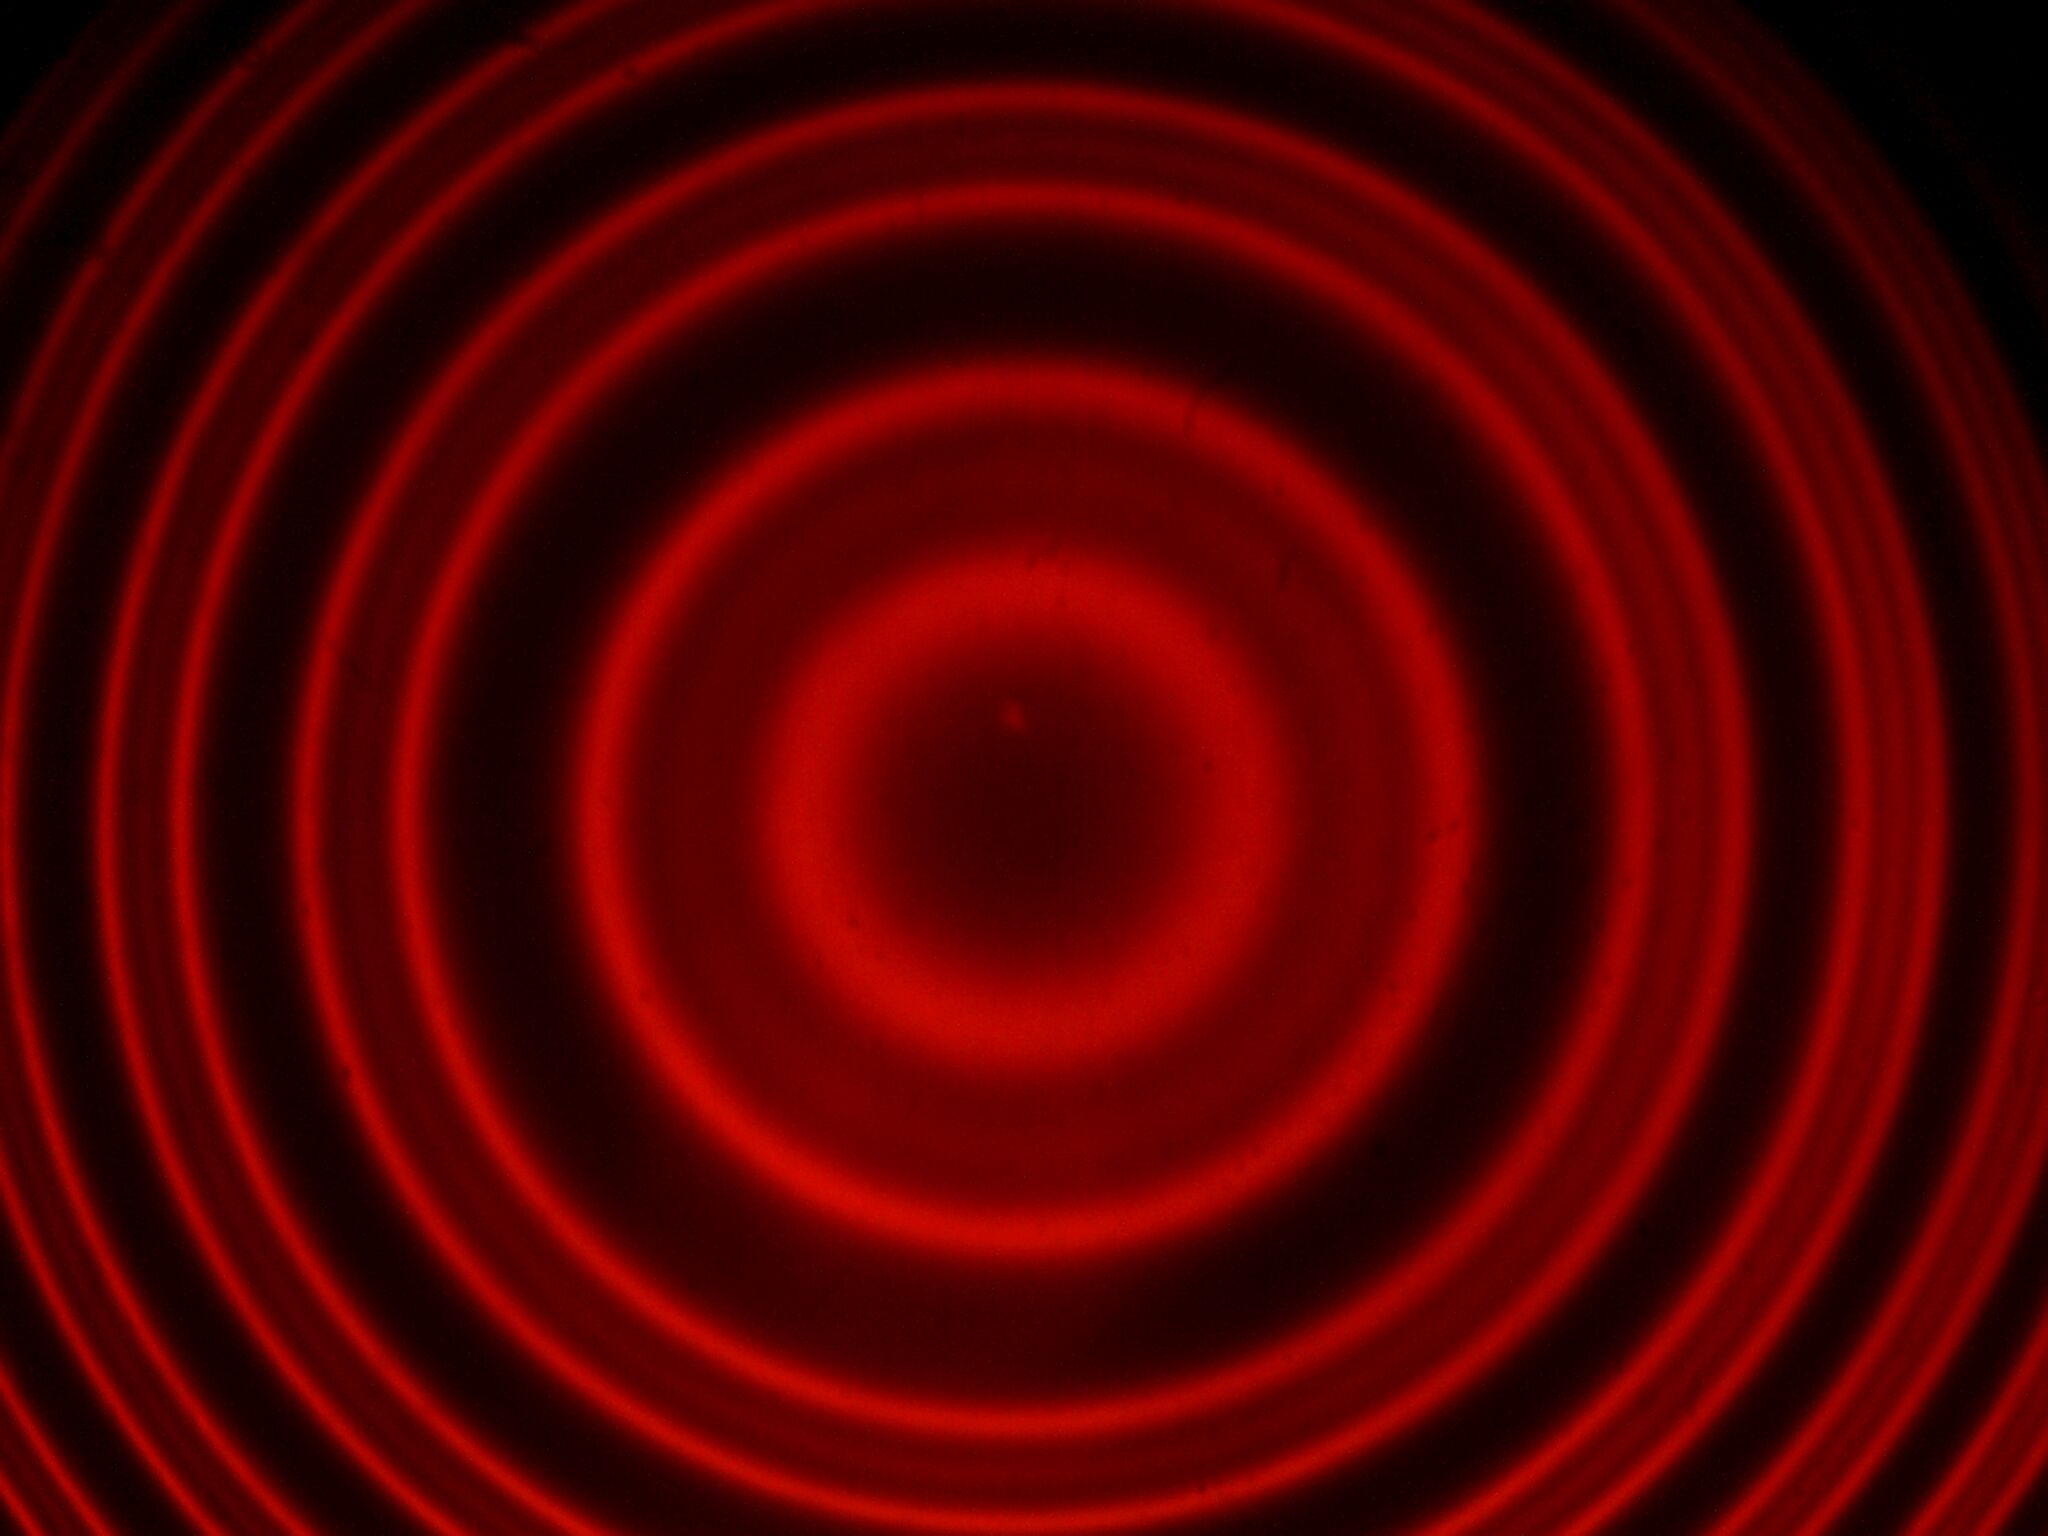
\includegraphics[width=\textwidth]{images/Capture_820.bmp.jpg}
			\caption{$I = \SI{7.01(1)}{\ampere}$}
			\label{fig:red_I7.01}
			\vspace{0.5\baselineskip}
		\end{subfigure}
		\begin{subfigure}{0.48\textwidth}
			\centering
			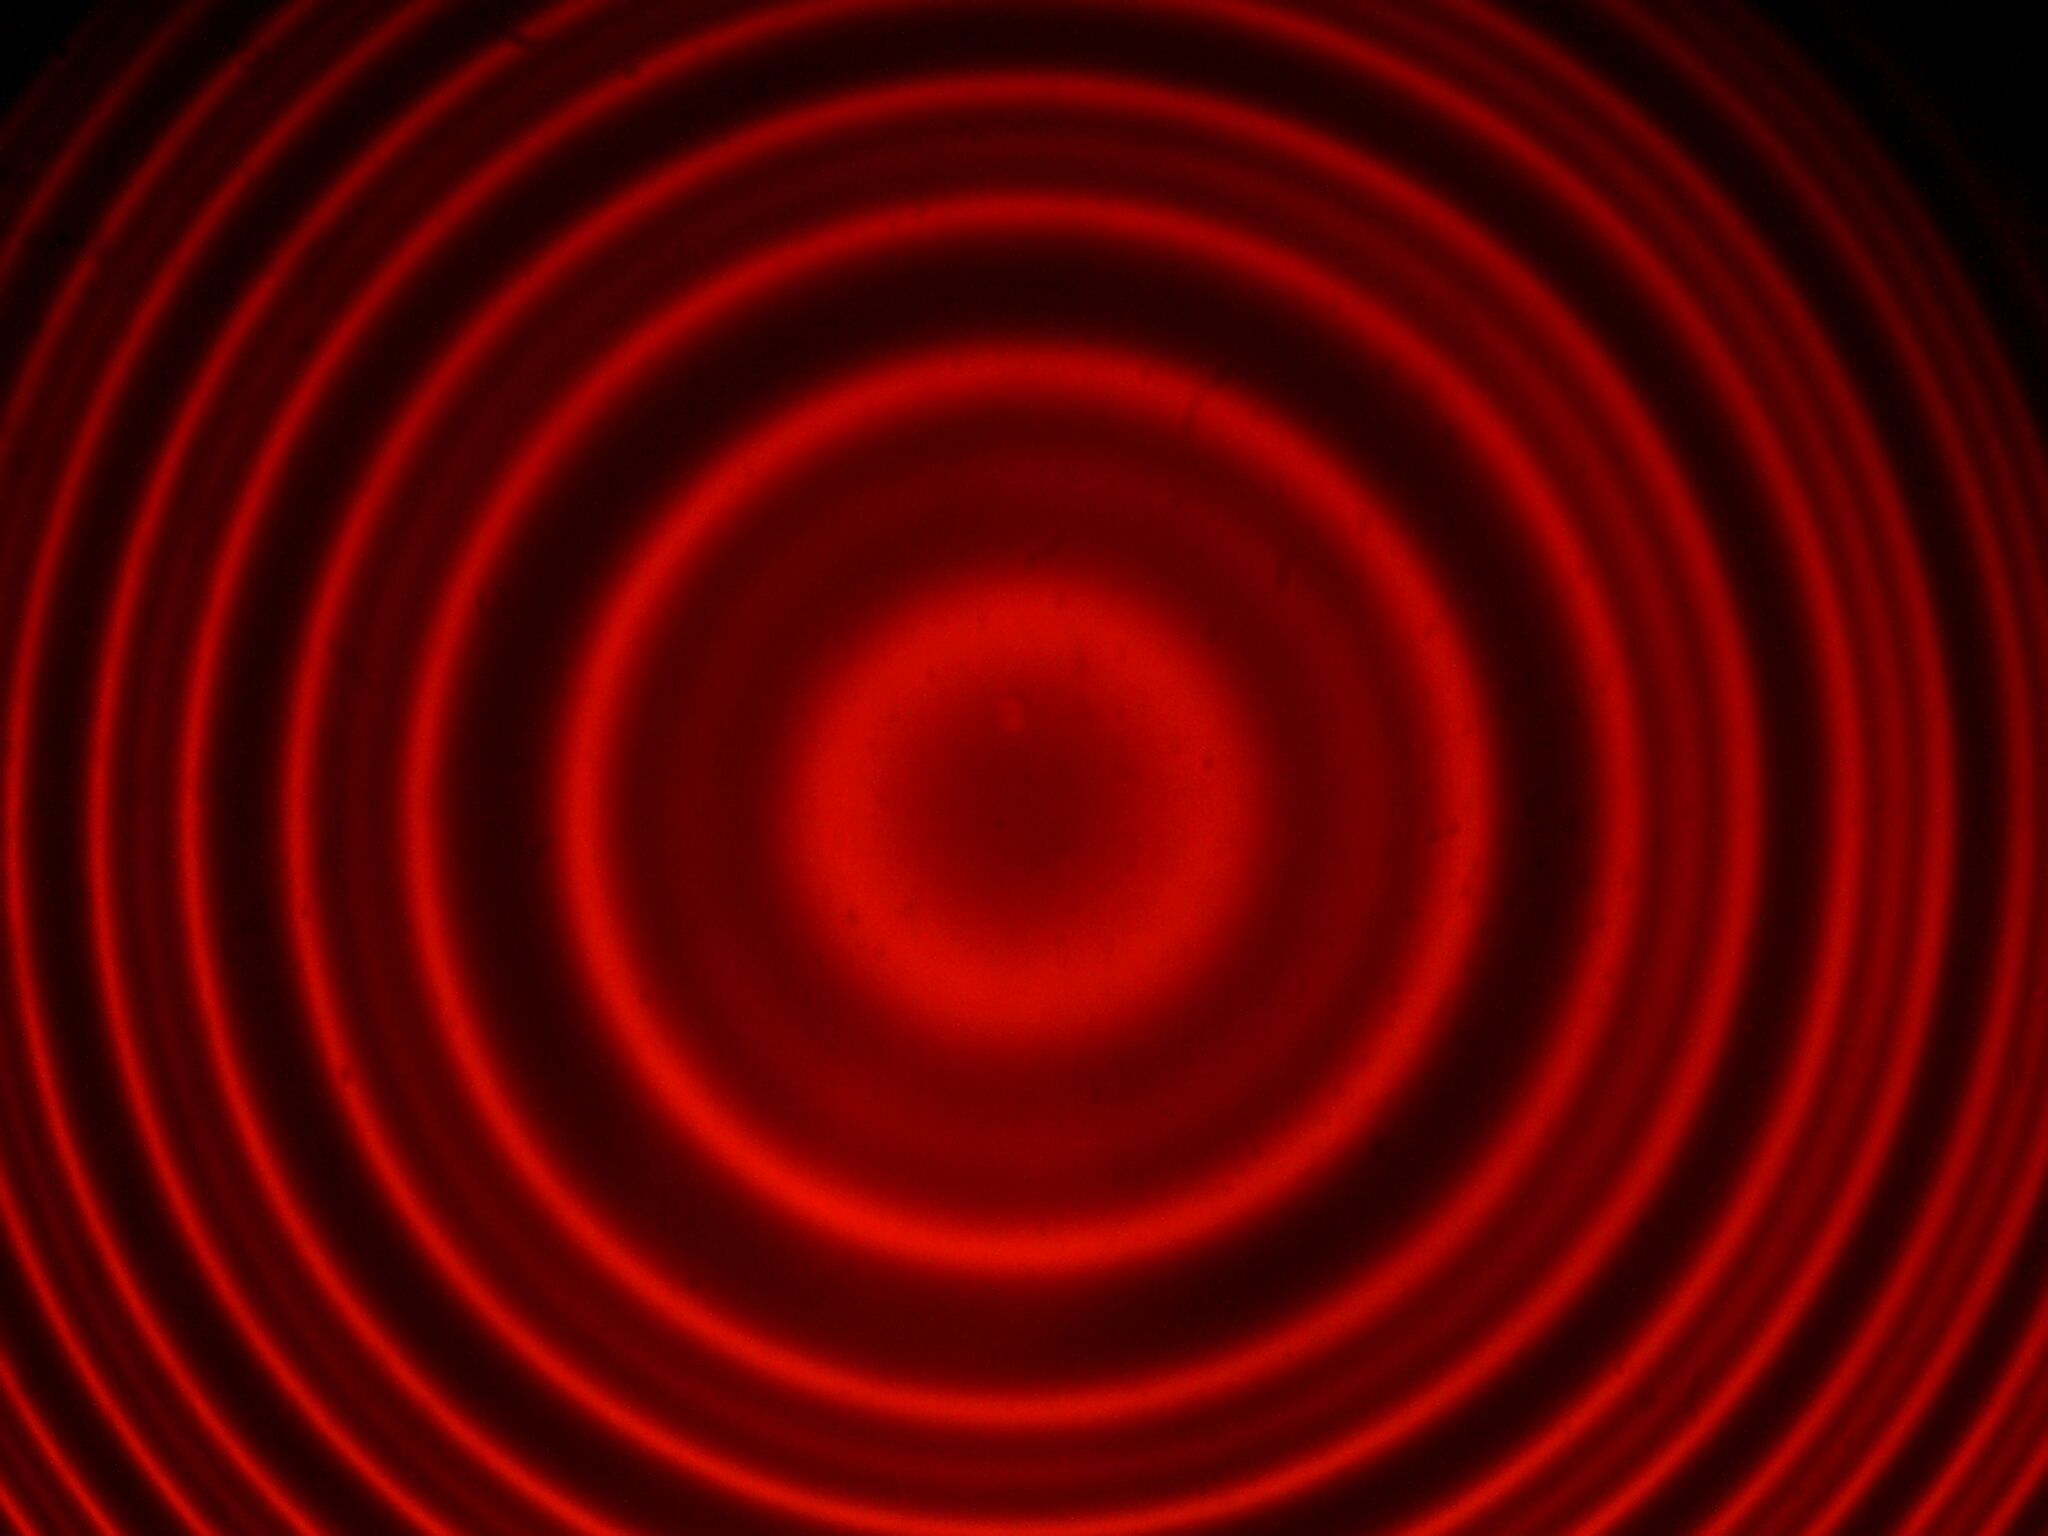
\includegraphics[width=\textwidth]{images/Capture_821.bmp.jpg}
			\caption{$I = \SI{8.78(1)}{\ampere}$}
			\label{fig:red_I8.78}
		\end{subfigure}
	    \caption{Messungen}
	    \label{fig:tv4-messungen}
	\end{figure}
	\newpage
	Als Messreihe haben wir:
	\todo{messreihe}
	\newpage
	

